%%%%%%%%%%%%%%%%%%don't forget if needed %%%%%%%%%%%%%%%%%%%%%
%\section[toc version]{title version%
%              \sectionmark{head version}}
%\sectionmark{head version}
%%%%%%%%%%%%%%%%%%%%%%%%%%%%%%%%%%%%%%%%%%%%%%%%%%%%%%%%%%%%%%
\def\titcourt{Numerical comparison of basal and lateral melting of phase change material}
\def\titlong{Numerical comparison of basal and lateral melting of phase change material}
%%%%%%%%%%%%%%%%%%%%%%%%%%%%%%%%%%%%%%%%%%%%%%%%%%%%%%%%%%%%%%%%
\chapter[\titlong]{\titlong%
              \chaptermark{\titcourt}}
\chaptermark{\titcourt}
\label{chap-MELTING-ANALYSIS}
%%%%%%%%%%%%%%%%%%%%%%%%%%%%%%%%%%%%%%%%%%%%%%%%%%%%%%%%%%%%%%%%
%%%%%%%%%%%%%%%%%%%%%%%%%%%%%%%%%%%%%%%%%%%%%%%%%%%%%%%%%%%%%%%%

We have performed extensive validations of our numerical method in Chapters \ref{chap-NATCONV} and \ref{chap-MELTING}.
Very good agreements were noticed for all validation tests against well-known benchmark cases and the robustness of the algorithm was proven by simulating challenging configurations.
We now use the code as an investigation tool to analyse the phase-change process during the melting stage.
We consider a square cavity of height $H$ filled with n-octadecane PCM and pay a closer attention to the temporal evolution of different physical parameters of the system. 
\begin{figure}
	\begin{center}
		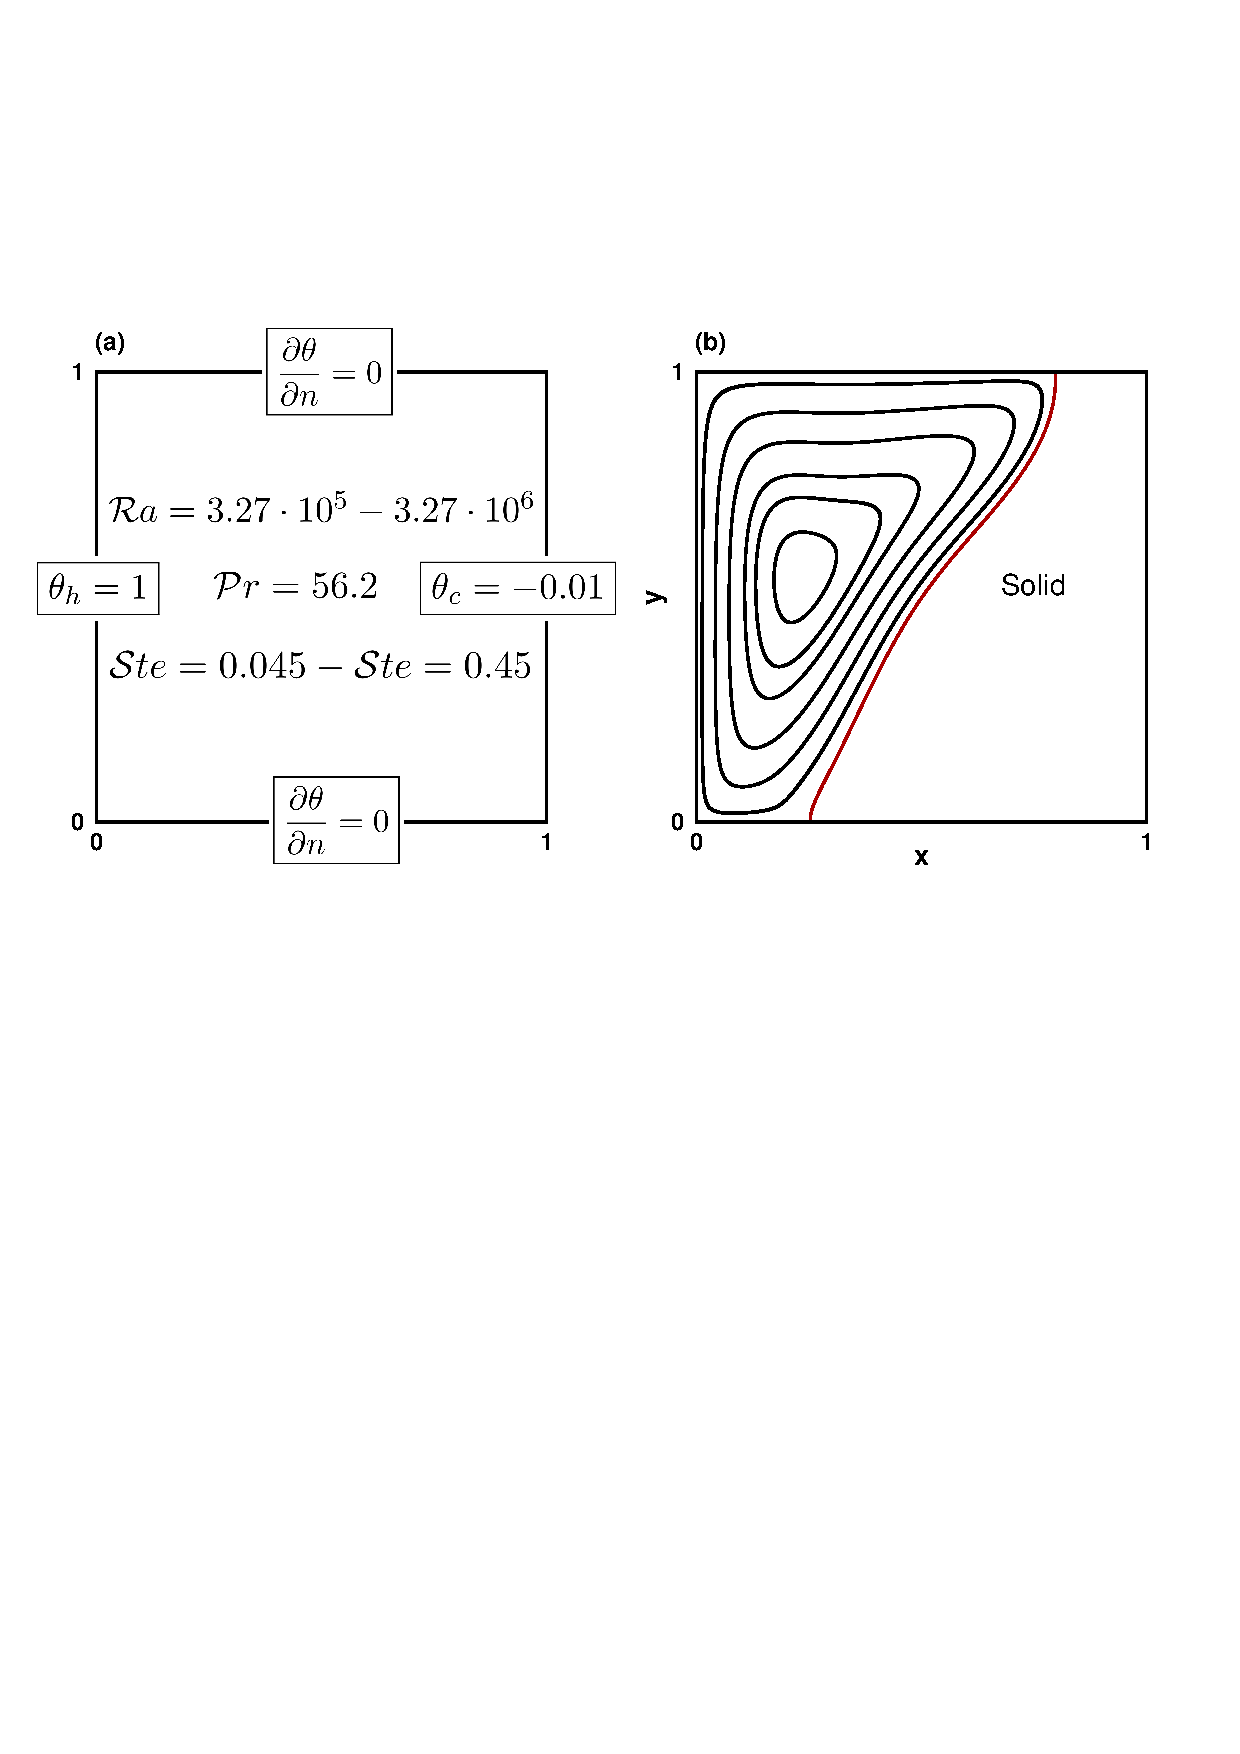
\includegraphics[width=.95\textwidth]{\figpath/Fig_cap_melting_basal/Scheme-melt-lat} \\
		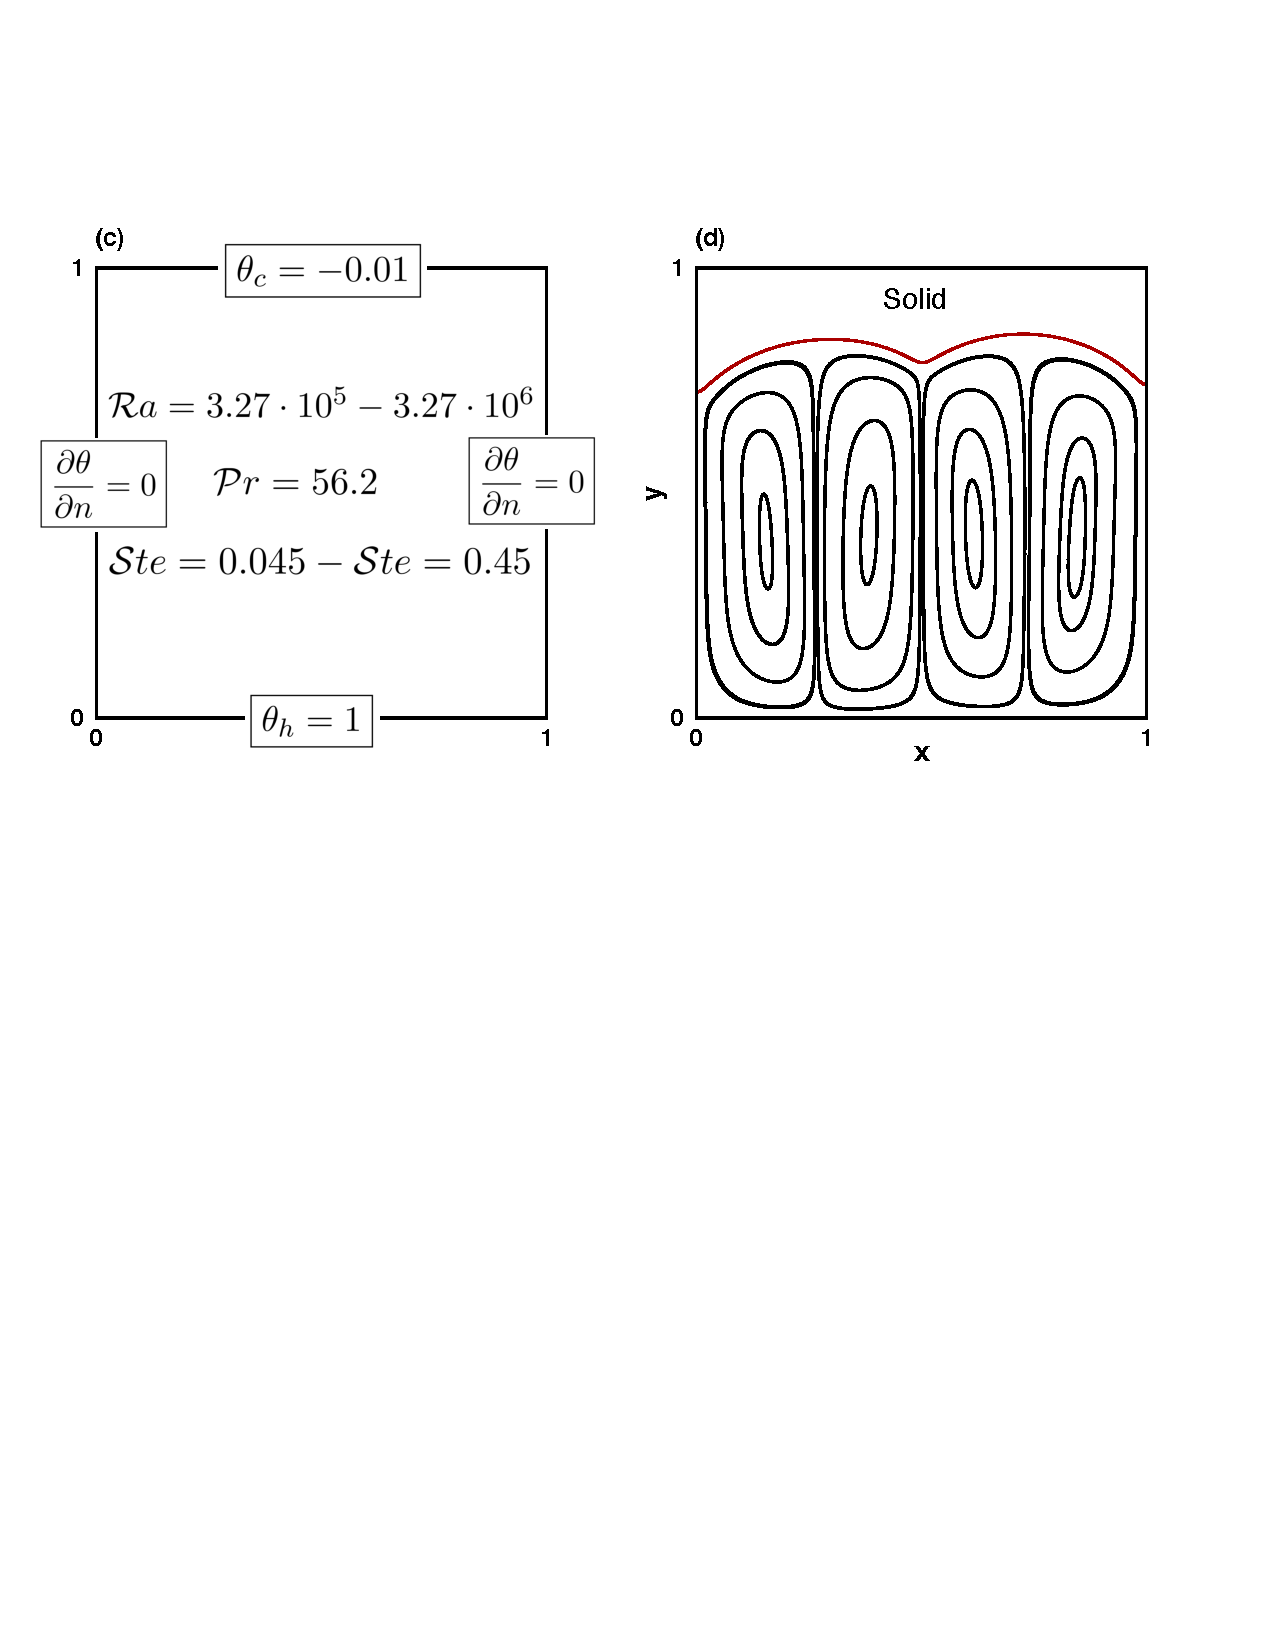
\includegraphics[width=.95\textwidth]{\figpath/Fig_cap_melting_basal/Scheme-melt-basal}
	\end{center}
	\caption{Comparison between lateral and basal melting. Sketch of the computational domain and boundary conditions for LM (top) and BM (bottom) cases. Streamlines (panels b and d) and solid-liquid interface (solid red lines).} \label{fig:melt-scheme}
\end{figure}

Two classes of convective melting systems are of interest in this chapter: \textbf{(i)} lateral melting (LM) or \textbf{(ii)}  basal melting (BM).
As far as \textit{(i)} is concerned, the PCM is subject to heating from the left side of the cavity, whereas for BM case the PCM is heated from the bottom within top melting boundary.
The comparison of both cases is appealing since the dynamics of the melting is known to be fundamentally different for each of the two cases.
The investigated configuration, the shape of the interface and the streamlines in the liquid phase are illustrated in Fig. \ref{fig:melt-scheme}. 
LM case (top) exhibits a mono cellular pattern while Rayleigh-B�nard-like convection cells are features of the BM case (bottom). 

\noindent LM case could be representative of building applications, solar collectors or other thermal energy storage systems. 
In the frame of building applications, bricks made of PCM melt because of differences between outdoor and indoor temperatures and store the energy in the form of latent heat.
\cite{barreneche2016situ} showed that a wall made of PCMs allows to reduce the temperature peak of about $20 \%$.
With regard to LM configurations, analytical investigation of \cite{bejan1989analysis} and scaling analysis of \cite{jany1988scaling} permitted to describe the heat transfer during the melting by the mean of $\Nuss$-$\Ray$ correlation and will be used in the present work. 
The second class, BM case, refers to passive temperature control for electronic devices or for a long list of geophysical problems,
such as lava lakes, thermal convection in magma chambers, or ice-melt lakes. 
In contrast with LM case, notwithstanding linear and weakly non-linear instability analysis based on a vanishingly small Stefan number assumption \citep{vasil2011dynamic}, exact expression of $\Nuss$ and $L_f$ from purely theoretical work are not available during the convective regime due to the important non-linearities of the dynamics.
Some comparisons with theories \citep{malkus1954heat,grossmann2000scaling} made in the frame of Rayleigh-B�nard convection flow have been however carried out \citep{esfahani2018basal,madruga2018dynamic,favier2019rayleigh}.
In this work, we develop a scale analysis during the so-called 'linear regime', which occurs between the onset of convective and oscillating flows.

The current work is scoped to offer a comprehensive comparison between LM and BM configurations.
We analyse first the time evolution of the LM process through a scale analysis in Sec. \ref{sec-melting-lateral}.
Second, the BM case is studied in Sec. \ref{sec-melting-basal} with theoretical descriptions of the heat transfer involving during the melting.
Finally, a comparison between the two cases is presented in Sec. \ref{sec-compare-LM-BM} and we suggest some practical applications reflecting our analysis.

\section{Lateral melting of n-octadecane PCM. Case LM}  \label{sec-melting-lateral}
We consider the physical properties of n-octadecane given in Tab. \ref{tab-param-PCM} and investigate
different height $H$ of the cavity and different value of $\delta T$, to assess the influence of the $\Ray$ number.
The numerical configuration is sketched in Fig. \ref{fig:melt-scheme}a.
$\Ray$ numbers ranging from $3.27 \cdot 10^5$ to $3.27 \cdot 10^6$ are investigated.
We note that for the range of $\Ray$ and $\Ste$ numbers of interest, the assumption of $(\beta \times \delta T) \ll 0.01$ for the Boussinesq approximation, is verified.
A second dimensionless time $\tau$ related to the analytical correlation of \cite{jany1988scaling} is introduced:
\begin{equation}
\label{eq-adim-tau}
\tau = \Ste \times \mathcal{F}o = \Ste \times \frac{\alpha t_{\varphi}}{H^2}  = \frac{\Ste}{\Prd} \times t,
\end{equation}
where $\mathcal{F}o$ is the Fourier number. 

\subsection{Analysis of the time evolution of the melting process} \label{subsec-time-evol-lat}

We start by describing the time evolution of the melting process for the lowest value of the Stefan and Rayleigh numbers, i.e $\Ste = 0.045$ and $\Ray = 3.27 \cdot 10^5$.
We are interested in a slow melting of the PCM to capture the transitions between the regimes described by \cite{jany1988scaling}, mainly the onset of the convective regime.

\noindent At $\tau=0$, the material is solid and the initial temperature is set to $\theta_0=-0.01$ everywhere inside the cavity. 
Then, the temperature of the left wall is progressively increased to $\theta_h=1$, while the right wall is maintained at the same cold temperature $\theta_c=-0.01$. 
The material starts to melt, with a melting front (identified by the iso-line $\theta=\theta_f=0$) propagating from the left to the right side of the domain. 
\begin{figure}
	\begin{center}
		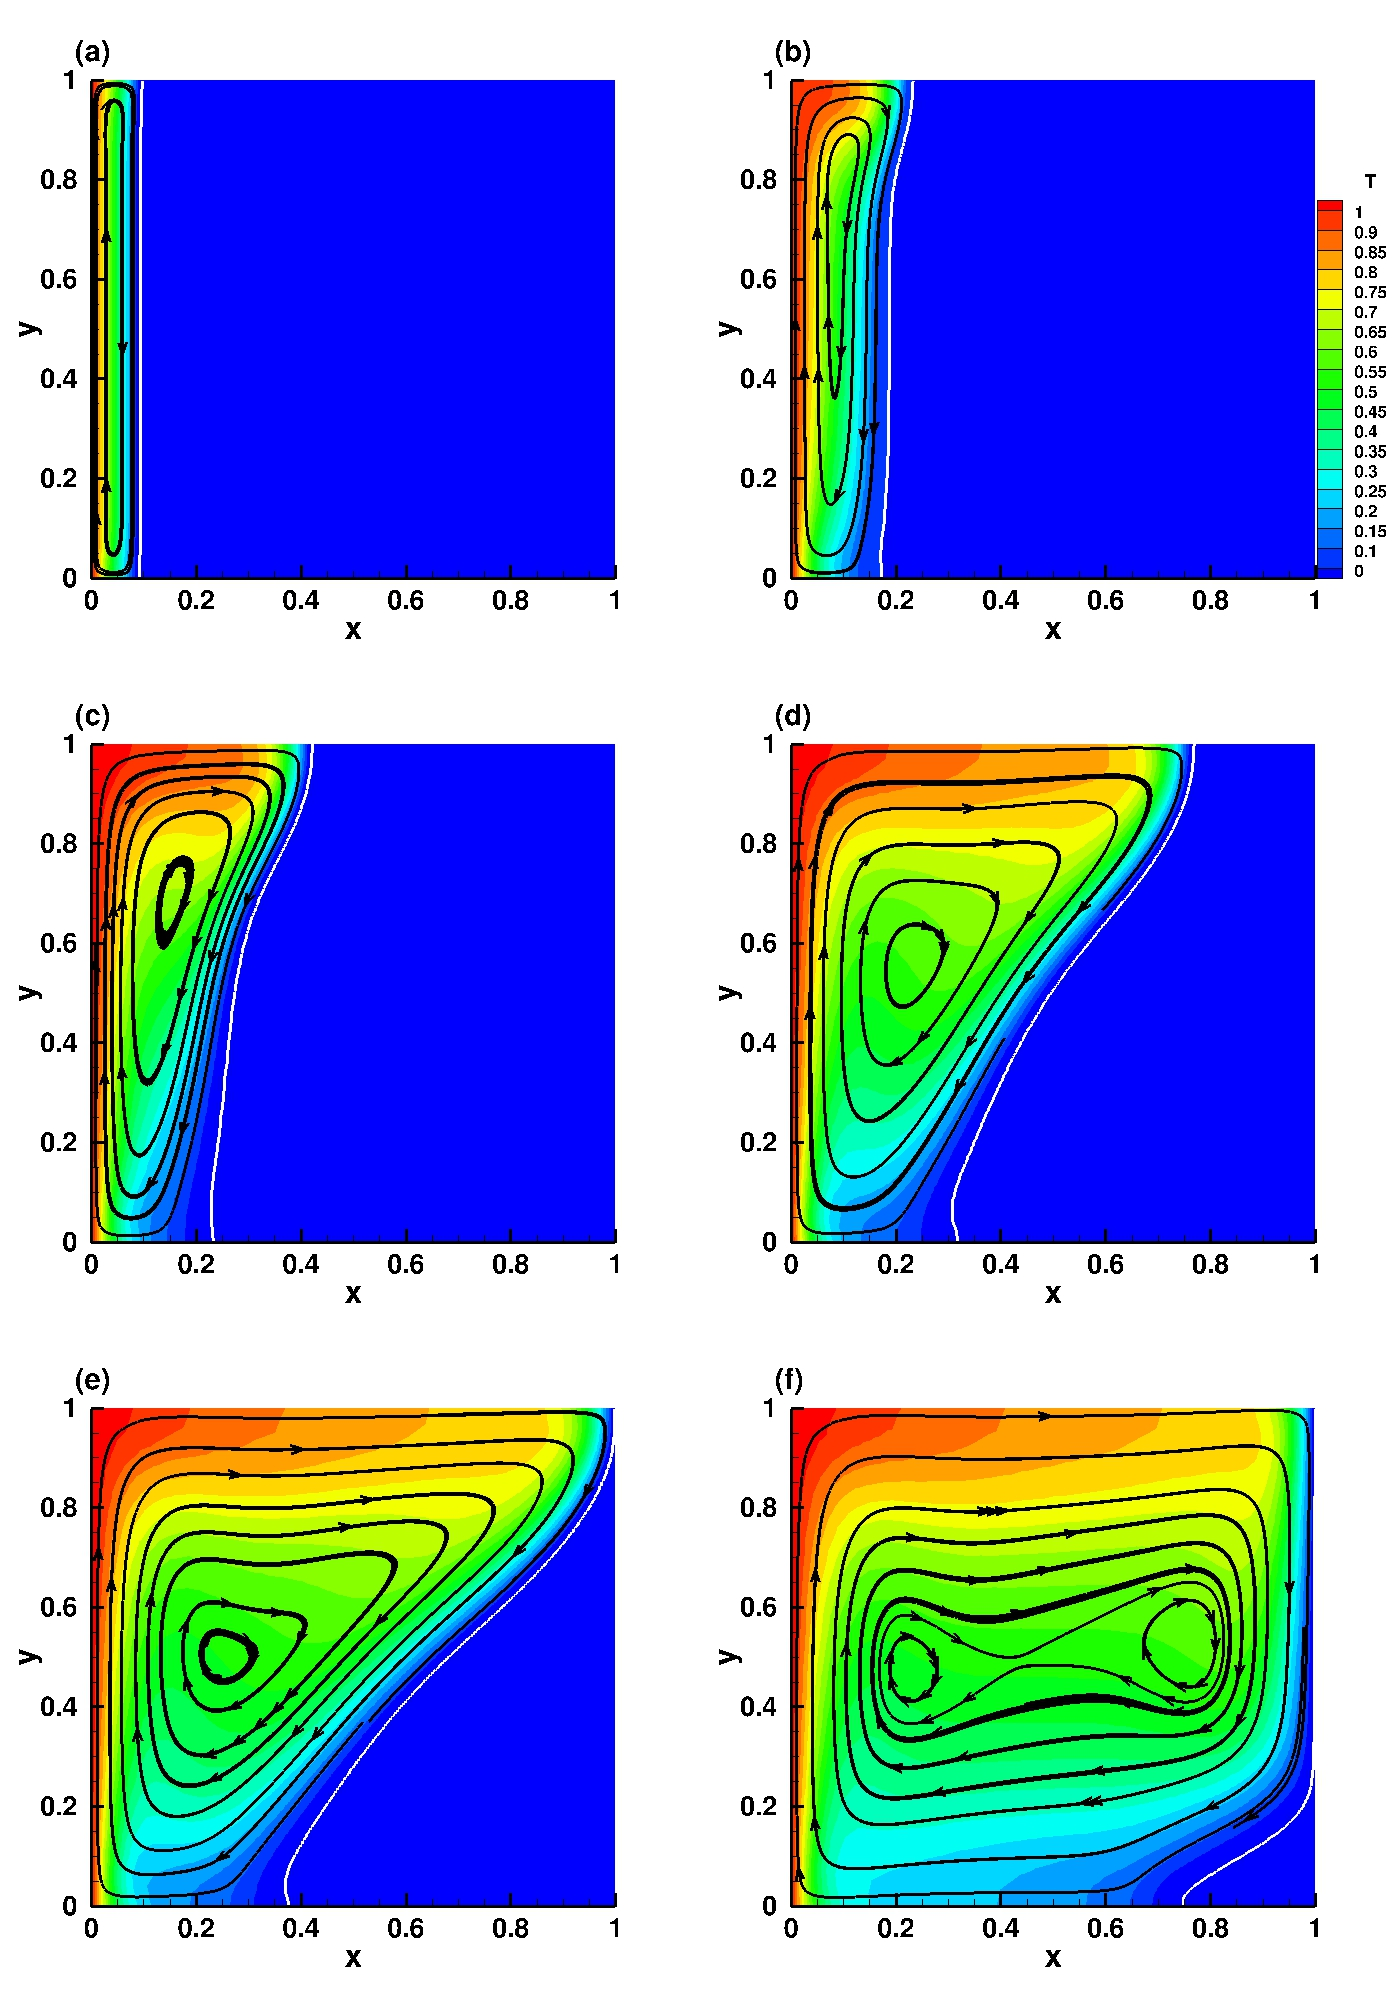
\includegraphics[width=.9\textwidth]{\figpath/Fig_cap_melting_basal/MELT_cavity_field}
	\end{center}
	\caption{Temperature iso-lines, streamlines in the fluid phase, and phase-change interface. The solid part is represented in blue and corresponds to the region of temperature $\theta \leq \theta_f=0$. Time instants (panels  a to f): $\tau=0.004; 0.016; 0.032; 0.063; 0.08; 0.2$. $\Ray = 3.27 \cdot 10^5$, $\Prd = 56.2$ and $\Ste = 0.045$.
		}\label{fig:melt-field}
\end{figure}
Snapshots of the time evolution of the phase-change system are given in Fig. \ref{fig:melt-field} for representative time instants.
Panels (a) to (f) offer the streamline showing the clockwise recirculation of the fluid, the melting front, and the temperature distribution (the solid phase is denoted by the blue region) for a comprehensive description of the evolution of the system. 
We can easily identify three different regimes describing the time evolution of the melting process. 

\begin{itemize}
	\item From $\tau=0$ to $\tau =0.004$ (Fig.  \ref{fig:melt-field}a), we note the vertical shape of the melting front, well predicted by the classical conduction model of \cite{stefan1891theorie}. This indicates that, at this stage, heat transfer is dominated solely by conduction.
	
	 \item Between $\tau =0.016$ to $\tau =0.032$ (Fig.  \ref{fig:melt-field}b), the natural convection in the fluid phase starts to alter the shape of the melting front.
	A mixed conduction and convection regimes rule the heat transfer. 	
	Convective flow mainly affects the upper part of the fluid motion, while conduction is still dominating in the lower part. As the volume thermal expansion coefficient $\beta$ is positive, we expect a clockwise circulation of the liquid inside the convection cell, as noted by \cite{jany1988scaling}.
	This also makes the liquid-solid interface to move faster at the top of the cavity, explaining the deformed shape of the melting front, which is a signature of the convection effects  (see also \cite{kowalewski2004phase}). 
	
	\item After $\tau=0.032$ (Fig.  \ref{fig:melt-field}c-d), natural convection dominates the heat transfer process and impacts radically the solid-liquid interface shape and motion.
	The melting front line exhibits four distinct regions characterized by different slopes with respect to the vertical axis. The largest slope is observed at the top of the cavity and is related to the particular shape of the convection cell. Note that top and bottom parts of the interface are normal to the cavity boundaries because of the imposed adiabatic boundary conditions.

	\item After $\tau =0.08$  the melting front is nearly touching the right wall of the cavity, firstly at the top (Fig.  \ref{fig:melt-field}e) of the cavity. The melting process continues and the fluid progressively fills the cavity, with a melting front  deforming to a vertical line. The  simulation of the melting process is stopped at $\tau =0.2$ (Fig.  \ref{fig:melt-field}f), when it is numerically difficult to separate the melting front from the right wall boundary. At this time instant,  the fluid fraction reaches the value of $0.95$ and  the melting of the PCM is considered to be complete, even though a small region of solid PCM remains at the lower right bottom of the cavity. Note from Fig.  \ref{fig:melt-field}f the existence in the fluid  of two recirculating zones instead of a single one observed during previous stages.
	
\end{itemize}

\subsection{Scale analysis of the melting} \label{sec:scaling anal}

We further analyse each of the three regimes cited previously and identify the proper scales of the phenomenon.
The (dimensionless) location of the interface will be denoted by $\Gamma_i$.
Immediately after the melting starts (see Fig. \ref{fig:melt-field}a), the melted PCM occupies a thin enclosure of height $H$ and width $\Gamma_i$.
In such configuration, the temperature varies linearly between the two sidewalls and the heat transfer is essentially ruled by conduction. 
The fluid phase is almost motionless and the horizontal heat flux across the incipient melting PCM is balanced by the enthalpy absorbed at the interface.
At the solid-liquid interface, the energy balance condition which takes into account the released latent heat and the discontinuity of heat flux between the solid and the liquid can be handled by the following Stefan condition:
\begin{eqnarray} \label{eq:Ste-condition}
	\theta (x=\Gamma_i) &=& \theta_f =  0, \\ \nonumber
	\frac{\partial \Gamma_i}{\partial t} &=& - \frac{\Ste}{\Prd} \frac{\partial \theta}{\partial x},
\end{eqnarray}

\noindent Since the temperature field during the conduction regime is quasi-steady, Eq. \ref{eq:Ste-condition} which is linear could be approximated by
\begin{equation}
    \frac{\partial \Gamma_i}{\partial t} \approx - \frac{\Ste}{\Prd} \frac{\theta_f - \theta_h}{\Gamma_i} \approx  \frac{\Ste}{\Prd} \frac{1}{\Gamma_i}.
\end{equation}

\noindent The location $\Gamma_i$ of the interface is consequently given by
\begin{equation} \label{eq-cond-evol}
   \Gamma_i = \sqrt{2 \times \frac{\Ste}{\Prd} t} = \sqrt{2 \tau}.
\end{equation}

\noindent Moreover, the Nusselt number can be evaluated using the same assumption,
\begin{equation}
   \Nuss= \int_0^{1} \left. \frac{\partial \theta}{\partial x} \right|_{x=0} dy = \frac{1}{\Gamma_i} = ({2 \tau})^{-1/2}.
\end{equation}

\noindent To summarize, during the very first stage of the melting, when the heat transfer is led by conduction, the time evolution of the liquid fraction (given by the location of the interface) and the Nusselt number could be approximated by
\begin{eqnarray} \label{eq-Nu-Lf-Corr-Lat}
	L_f &\sim& (2 \tau)^{1/2}, \\ 
	\Nuss &\sim& (2 \tau)^{-1/2}.
\end{eqnarray}

\begin{figure}
	\begin{center}
		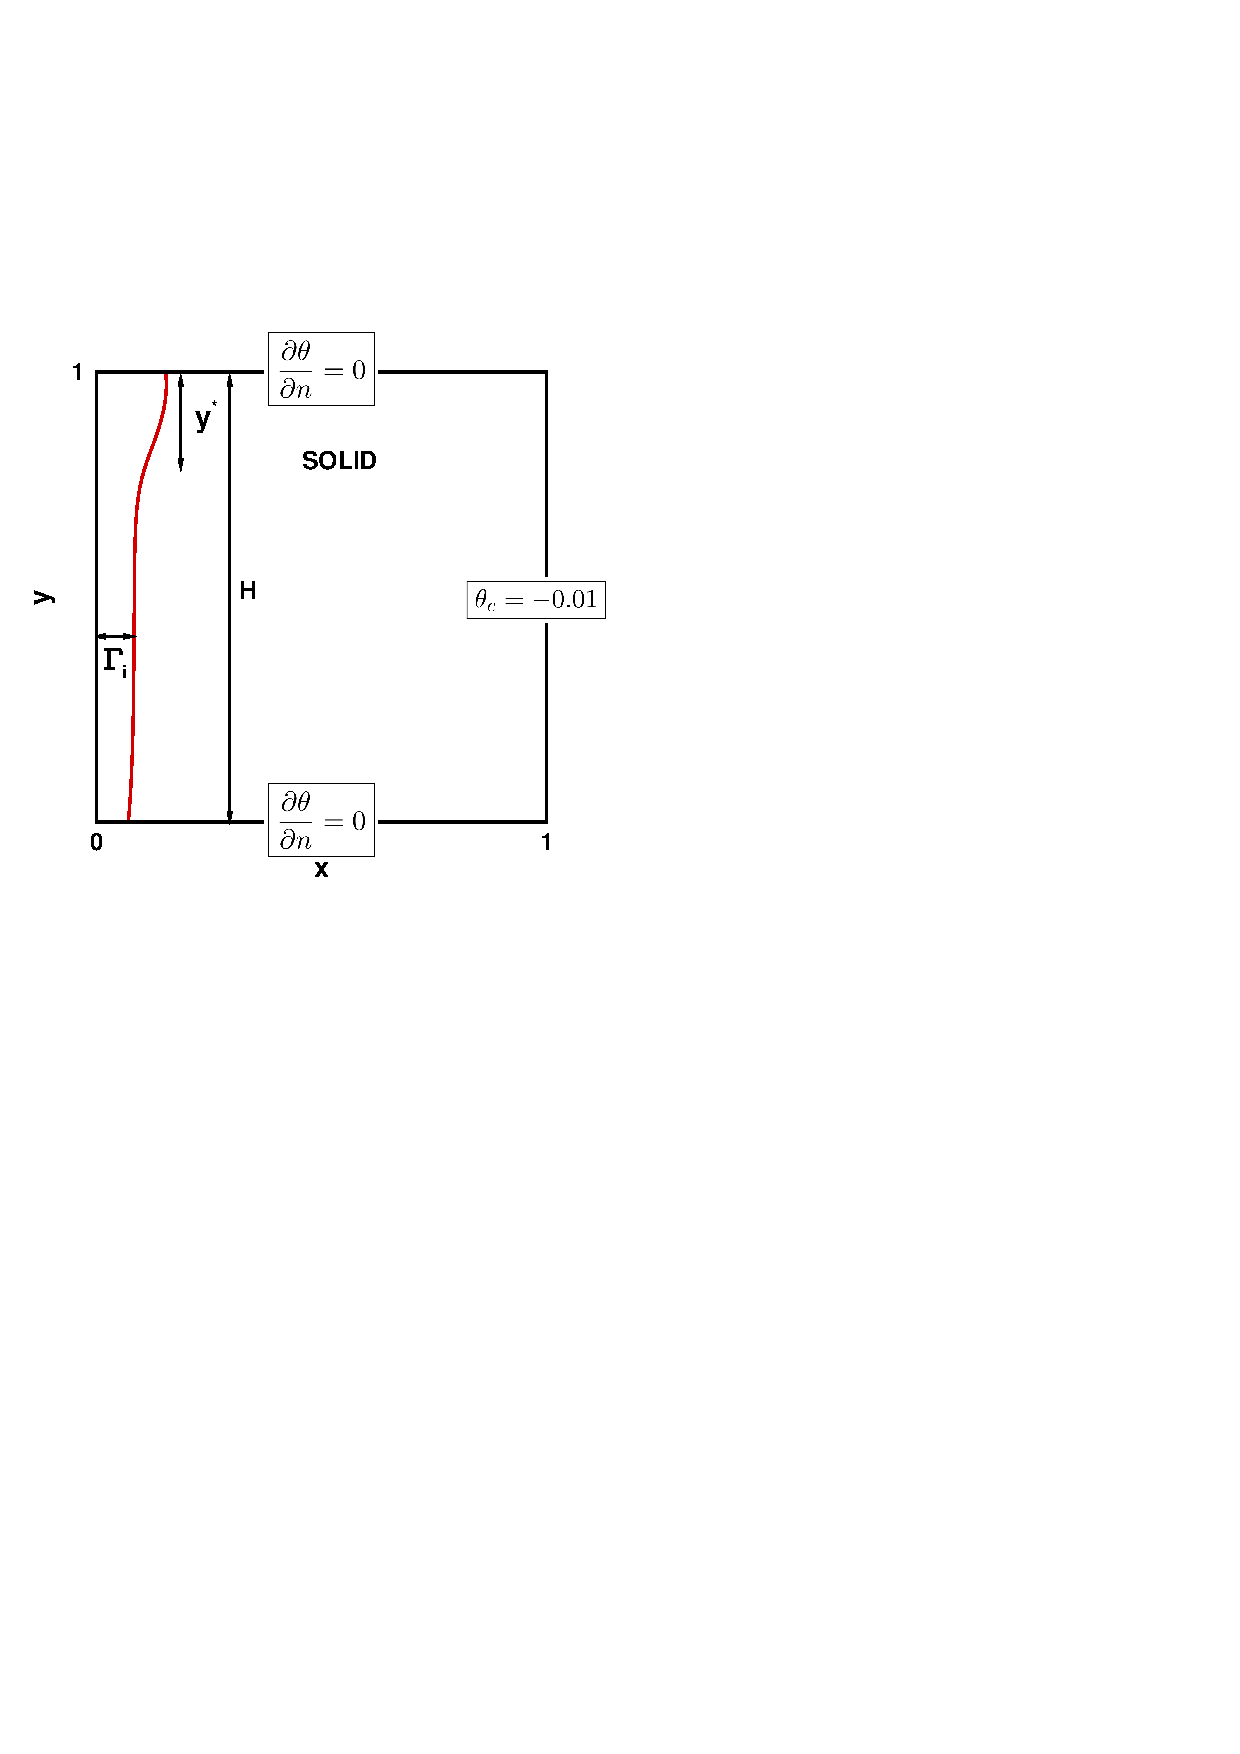
\includegraphics[width=.5\textwidth]{\figpath/Fig_cap_melting_basal/MELT_Regime_evol}
	\end{center}
	\caption{Illustration of the mixed regime by \cite{jany1988scaling}. Solid red line is the solid-liquid interface, $\Gamma_i$ represents the location of the interface and $y^*$ denotes the height of fluid impacted by the emerging convective flow.}\label{fig:melt-scheme-regime}
\end{figure}

While the melting continues to expand to the right side of the domain, a natural convection flow emerges from the top of the cavity since we have a clockwise recirculation of the flow in the liquid phase (see Fig. \ref{fig:melt-scheme-regime}).
Turning back to the energy Eq. \ref{eq-energ} in the liquid phase  (i.e. $C = K = 1$), three distinct effects could be identified:
\begin{equation}
	\underbrace{\frac{\delta \theta}{t}}_{Inertia} \quad \underbrace{v \frac{\delta \theta}{H}}_{Convection} \quad \underbrace{\frac{\delta \theta}{\Gamma_i^2}}_{Conduction},
\end{equation}

\noindent As $t$ increases, the inertia decreases in importance while the convection effect increases since it is proportional to $v$, and the conduction becomes more and more negligible with the increasing value of $\Gamma_i$ with time. 
\cite{jany1988scaling} described the convective heat transfer contributing during this regime by defining a Rayleigh number based on $y^*$ as $\Ray_{y^*} = \Ray \times y^{*3}$,
with $y^{*}$ the height of the melted zone altered by the convection flow as shown in Fig. \ref{fig:melt-scheme-regime}. 
At the bottom part of the cavity, the interface remains vertical by the effect of the conductive heat transfer.
The total Nusselt number during the mixed conduction-convection regime could be therefore approximated by \cite{jany1988scaling} approximation:
\begin{equation} \label{eq-Nu-conv-cond}
   \Nuss \sim (2 \tau)^{-1/2} + (2 \tau)^{3/2} \times \Ray.
\end{equation}

\noindent Eq. \ref{eq-Nu-conv-cond} indicates that the contribution of the conduction $\left(\sim 1/\sqrt{2 \tau}\right)$ decreases with the time while the convection one is increasing.

Finally, when the natural convection flow is fully developed and dominates the heat transfer along the vertical heated wall, with respect to the correlation of \cite{bejan2013convection}, the dimensionless thickness of thermal boundary layer is $\delta_{\theta} \sim \Ray^{1/4}$ (see also \cite{jany1988scaling}) and therefore the Nusselt number scale is
\begin{equation} \label{eq-Nu-Ra-LM}
   \Nuss \sim \Ray^{1/4}
\end{equation}

\noindent \cite{jany1988scaling} have proposed a more general single correlation, combining the regimes described previously:
\begin{equation} \label{eq-Nu-scale}
\Nuss(\tau) =  \frac{1}{\sqrt{2 \tau}} + \left[c_1 \Ray^{1/4} - \frac{1}{\sqrt{2 \tau}} \right]  \left[ 1 + \left(c_2 \Ray^{3/4}  \tau^{3/2}\right)^n \right]^{1/n}.
\end{equation}
The values of the constants were fitted from numerical data: $c_1 = 0.27$, $c_2 = 0.0275$, and $n=-2$. 

\cite{Okada1984} has also suggested from his experimental data the following correlation for $\Nuss$: %taking into account the foregoing presented regimes:
\begin{equation} \label{eq-corr-Okada}
	\Nuss = \left \{
	      %\begin{array}{ll}
	      \begin{aligned}
	      		\frac{1}{\sqrt{2 \tau}} \quad  &\text{if} \quad \tau \leq \tau_t, \\ 
	      		\frac{1}{\sqrt{2 \tau_t}} \left \{ 1 + C (\tau - \tau_t) \right \} \quad & \text{if} \quad \tau > \tau_t, \\
			c_1 \Ray^{0.266} \quad & \text{otherwise},
	       %\end{array}  
	       \end{aligned}
	\right.
\end{equation}
with the constant $c_1 = 0.234$ and the power $0.266$ fitted from experimental data, and $\tau_t$ the transition time from conduction to convection as discussed previously.

\noindent Predictions of Eqs. \ref{eq-corr-Okada} and \ref{eq-Nu-scale} are compared with our numerical results in Fig. \ref{fig:Nusselt} showing the time evolution of the Nusselt number at the left wall.
Our results perfectly fit with the theoretical prediction of \cite{jany1988scaling} and are also in good agreement with the experimental correlation of \cite{Okada1984}. 
The gap between the current simulation and the results of \cite{Okada1984} could be explained by the experimental heat loss mentioned by the author and the uncertainties of the experimental measurements.
The regimes described by the shape of the interface in Sec. \ref{subsec-time-evol-lat} could be featured by the temporal evolution of $\Nuss$:
\begin{enumerate}
	\item \textbf{The pure conduction regime} ($\Nuss \sim (2 \tau)^{-1/2}$) for $\tau  \gtrsim 0$ to $\tau \sim \Ray^{-1/2} =0.02$  (corresponding to Fig.  \ref{fig:melt-field}a).
	Since the temperature gradient has initially huge values because of the increase of the temperature of the left wall, the Nusselt number rapidly decreases during the first stage of the flow evolution. 
	The  signature of this conduction regime is the slow heat transfer characterized by a monotonic decrease of the Nusselt number.
	
	\item \textbf{The mixed conduction-convection regime}  ($ \Nuss \sim \tau^{-1/2} + \Ray\, \tau^{3/2}$) for $  0.02  \leq \tau \leq 0.05$ (illustrated in  Fig.  \ref{fig:melt-field}b).

	\item \textbf{The convection dominated regime} ($ \Nuss \sim \Ray^{1/4}$) for $\tau > Ra^{-1/2}$  (corresponding to Figs.  \ref{fig:melt-field}c-e).
	The plateau at the value of $\Ray^{1/4}$ corresponds to the pure convective transfer and is observed in Fig. \ref{fig:Nusselt} for $  0.05 \leq \tau \leq 0.1$. Numerical results show a slight decrease of $\Nuss$ in the final stage ($\tau \geq 0.1$), when the melting front starts to touch the right wall of the cavity (see Figs.  \ref{fig:melt-field}e-f). The correlation model is not valid for this late evolution of the melting process.
\end{enumerate}

\begin{figure}
	\begin{center}
		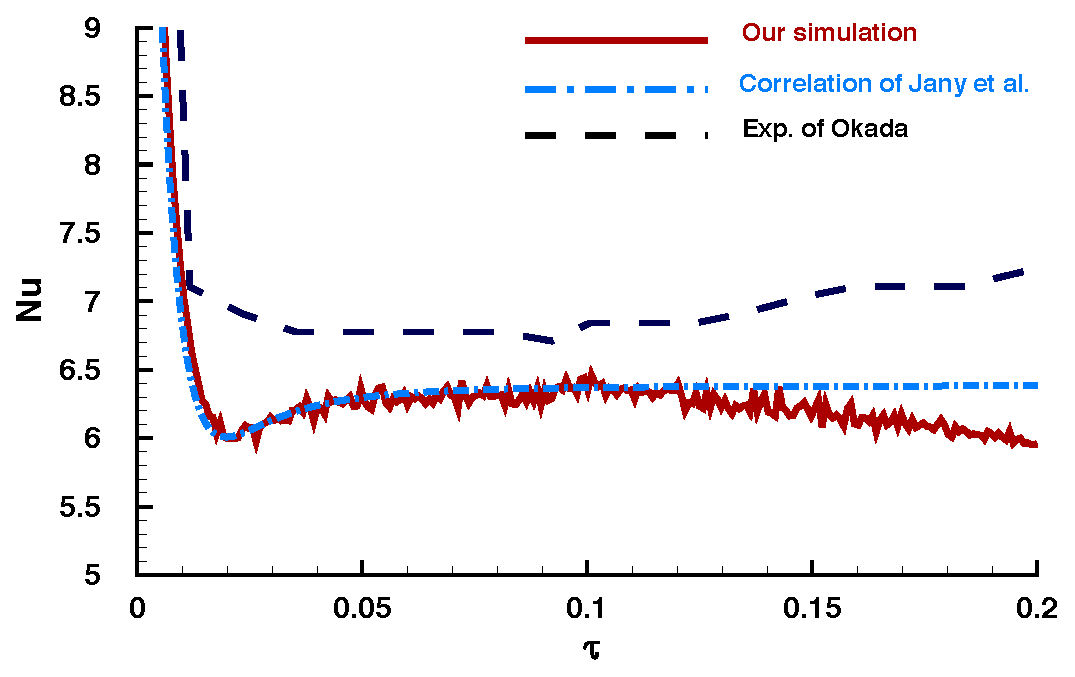
\includegraphics[width=.7\textwidth]{\figpath/Fig_cap_melting/fig06}		
	\end{center}
	\caption{Complete melting of the PCM. Time evolution of the average Nusselt number defined at the hot (left) wall (cf. Eq. \ref{eq-def-Nu}) (solid line). Comparison with the experimental results of  \cite{Okada1984} (dashed line) and the predictions using the correlation in Eq. \ref{eq-Nu-scale} suggested by \cite{jany1988scaling} (dash-dot line). $\Ray = 3.27 \cdot 10^5$, $\Prd = 56.2$ and $\Ste = 0.045$.}\label{fig:Nusselt}
\end{figure}


Another important basic quantity describing the melting process is the liquid fraction $L_f$.  
The time evolution of the liquid fraction (Fig. \ref{fig:Lf}a) displays three regimes during the melting process. $L_f$  initially grows as $\tau^{ 1/2}$, which is a typical law for a conduction-dominated heat transfer. Then, a linear temporal evolution is observed, until the melting front reaches the right wall.
This linear regime corresponds to the quasi-steady state observed in the evolution of the Nusselt number (Fig. \ref{fig:Nusselt}).

\noindent Using the asymptotic limits of Eq. \ref{eq-Nu-scale} for $ \tau \to 0$ (pure conduction) and $ \tau \to \infty$ (pure convection),  \cite{jany1988scaling} suggested the following correlation law for the time evolution of the liquid fraction:
\begin{equation} \label{eq-Lf-scale}
L_f(\tau) = \left[\left({\sqrt{2 \tau}} \right)^5 + \left(c_1 \Ray^{1/4}  \tau \right)^{5} \right]^{1/5},
\end{equation}
where $c_1=0.27$ is the same constant as in Eq. \ref{eq-Nu-scale}. 
We compare in Fig. \ref{fig:Lf}b our numerical results with the predictions based on Eq. \ref{eq-Lf-scale} within the validity domain of the analysis, \ie before the melting front reaches the right wall of the cavity. A very good agreement is found with theoretical predictions and also with previously published numerical results \citep{Wang2010}.

\begin{figure}[!ht]
	\begin{center}
		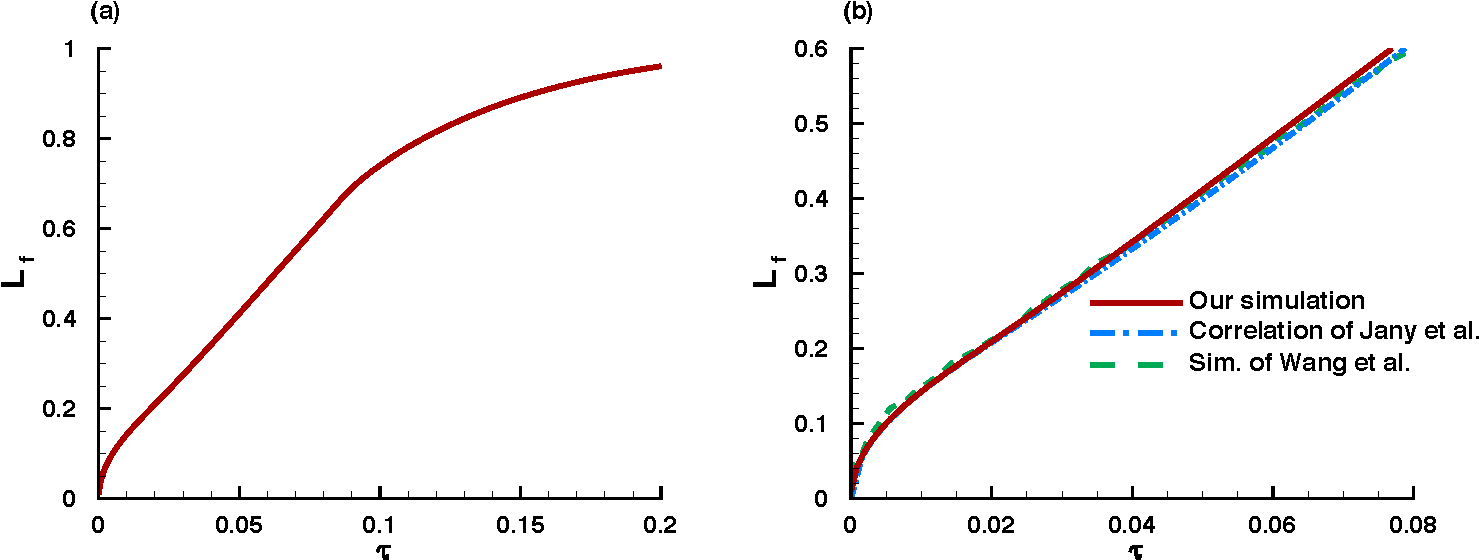
\includegraphics[width=0.9\textwidth]{\figpath/Fig_cap_melting/fig07}
	\end{center}
	\caption{Complete melting of the PCM. (a) Time evolution of the liquid fraction for the complete melting of the PCM. (b) Comparison of our results (solid line) with the numerical results of  \cite{Wang2010} (dashed line) and the predictions using the correlation (\ref{eq-Lf-scale}) suggested by \cite{jany1988scaling} (dash-dot line).}\label{fig:Lf}
\end{figure}


%%%%%%%%%%%%%%%%%%%%%ù
\subsection{Influence of the Rayleigh number}
%%%%%%%%%%%%%%%%%%%%%

\begin{figure}
	\begin{center}
		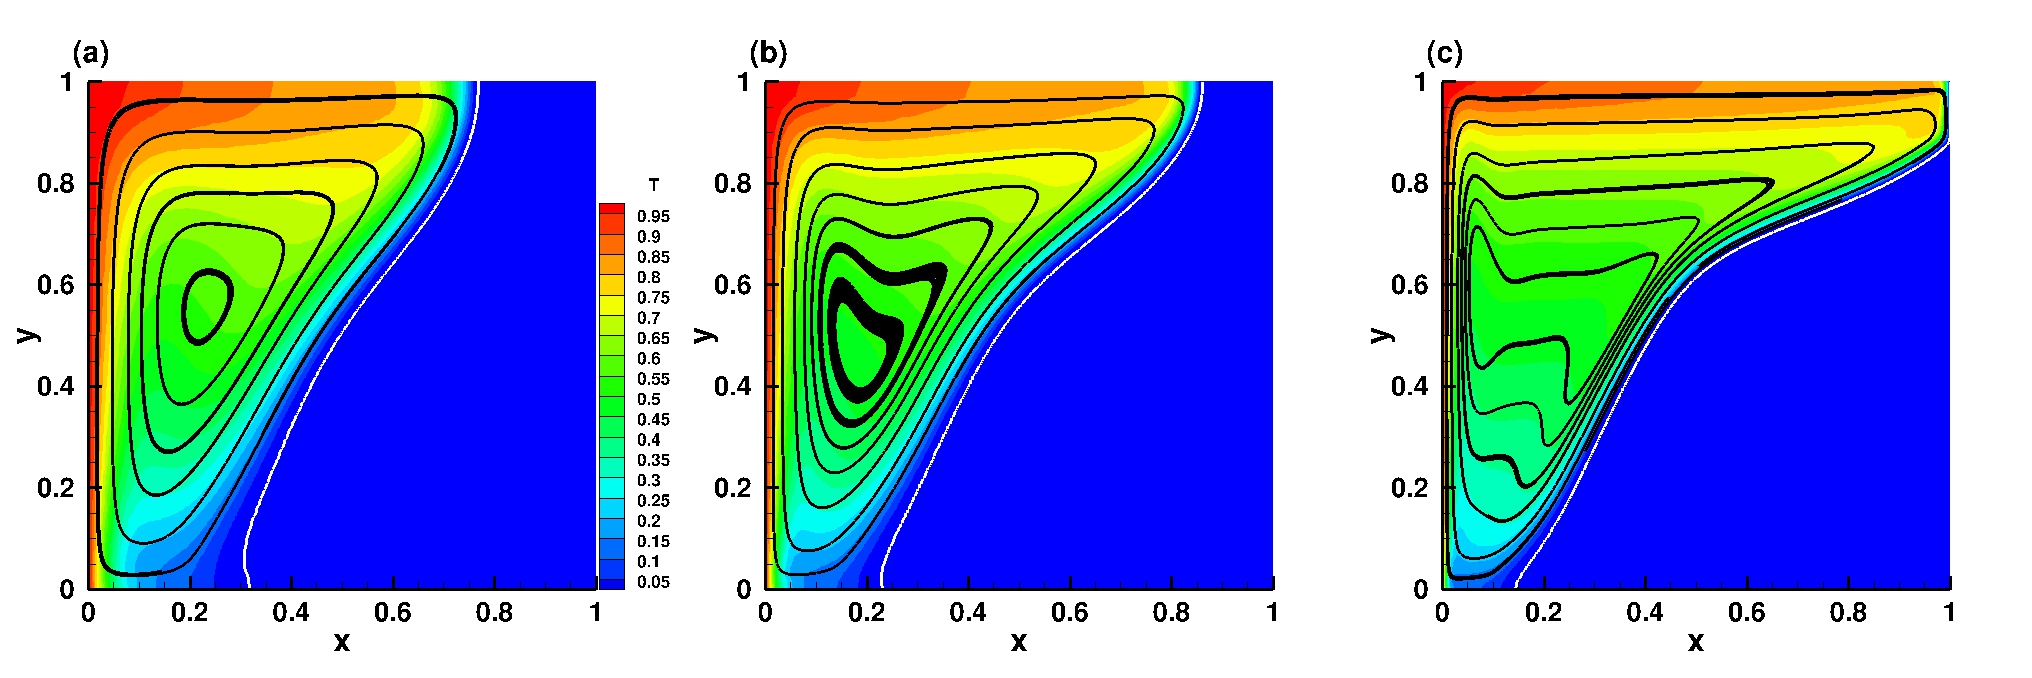
\includegraphics[width=\textwidth]{\figpath/Fig_cap_melting_basal/MELT_cavity_Ra_comp}
	\end{center}
	\caption{PCM melting at $L_f = 0.5$. Illustration of the temperature field, the streamlines, and the melting front for three $\Ray$ numbers: (a) $\Ray = 3.27 \cdot 10^5$ , (b) $\Ray = 1.62 \cdot 10^6$, and (c) $\Ray = 3.27 \cdot 10^6$.
	The $\Prd$ and $\Ste$ numbers are kept constant: $\Prd = 56.2$ and $\Ste = 0.045$.} \label{fig:melt-comp-Ra}
\end{figure}

To investigate the influence of the Rayleigh number on the evolution of the melting process, we performed different simulations by multiplying the initial value of $\Ray = 3.27 \cdot 10^5$ by a factor of 5 and 10, respectively. The exact values are: $\Ray = 1.62 \cdot 10^6$ and $\Ray = 3.27 \cdot 10^6$. 
First, we increase the height $H$ of the cavity by a factor of $\sqrt[3]{5}$ and $\sqrt[3]{10}$ and consider the same $\delta T$.
Thus the $\Ste$ number is kept constant.
Second, we increase the temperature difference parameter $\delta T$ by keeping $H$ constant.
It corresponds of an increased value of the Stefan number by a factor of $5 $ and $10$:
$\Ste = 0.223$ and $\Ste = 0.45$.

Snapshots of numerical solutions for $\Ray = 3.27 \cdot 10^5$,  $\Ray = 1.62 \cdot 10^6$ and  $\Ray = 3.27 \cdot 10^6$ at constant $\Ste$ number are given in Fig. \ref{fig:melt-comp-Ra}.
The colours correspond to the temperature distribution, the  black lines correspond to the streamlines and the white lines correspond to the solid-liquid interface.
Panels (a) to (c) depict the dynamics of the convective melting flow when half of the initial solid PCM ($L_f = 0.5$) have melted.
The top part of the interface moves faster while the bottom one is slowed by the increasing value of $\Ray$.
According to the Stefan interface condition in Eq. \ref{eq:Ste-condition}, at constant $\Ste$ and $\Prd$ numbers, the interface velocity is proportional to $\partial \theta / \partial n$, which is maximum at the top of the cavity because of the clockwise recirculation of the fluid explaining the observed trends.

Figures \ref{fig:Ra-Nusselt-H} and \ref{fig:Ra-Nusselt-deltaT} plot the temporal evolution of the liquid fraction $L_f$ (panel a),  and the average Nusselt number defined at the hot wall (panel b). 
The same heat transfer regimes described previously are observed for each case: conduction, mixed conduction-convection and convection.
We note that results are plotted with respect to physical time $t_{\varphi}$ instead of $\tau$, 
because we compare solutions with different values of $H$, which involves in the definition of the non-dimensional times $t$ and $\tau$, making them not relevant to compare solutions.

\noindent Figure \ref{fig:Ra-Nusselt-H}a indicates that increasing the Rayleigh number by keeping $\delta T$ constant induces a slower melting rate.
This is the expected behaviour since the size of the PCM is increased by a factor of 2, and the velocity $\vec u$ is decreasing to satisfy the condition $\Rey = 1$.
We note however a non-monotonic variation of the time necessary to melt a fixed value of fluid.
For instance, to achieve $L_f = 0.5$ (50\% of the volume is melted), an increase of $\Ray$ by a factor of $10$ leads to a growth of the time by a factor of $1.7$.
Nonetheless, when $\Ray$ is  $5$ times larger, the necessary time only increases by a factory of $2$.
This is most likely due to the non-linear intricacies of the problem and requires further investigation.
Furthermore, the Nusselt number reported in Fig. \ref{fig:Ra-Nusselt-H}b shows that the higher the Rayleigh number, the higher the Nusselt number.
This is consistent, since the temperature gradient is integrated along a greater heated wall. 

\noindent Figure \ref{fig:Ra-Nusselt-deltaT}a shows that by increasing the value of $\delta T$, and consequently increasing the Rayleigh number and the Stefan number, the PCM melts faster. 
We note that the height $H$ of the cavity is kept constant, hence the natural convection flow in the melted PCM is enhanced when the Rayleigh number keep increasing.
As a consequence, the convection-dominated regime is reached earlier, as shown by the shift of the minimum of the $\Nuss$ to lower values of $t_{\varphi}$ in Fig. \ref{fig:Ra-Nusselt-deltaT}b. 
This evolution is also observed for the liquid fraction. 
As expected, an increase of the Rayleigh number and the Stefan number is followed by an enhancement of the heat transfer during the melting, and consequently an improved efficiency of the PCM.
\begin{figure}
	\begin{center}
		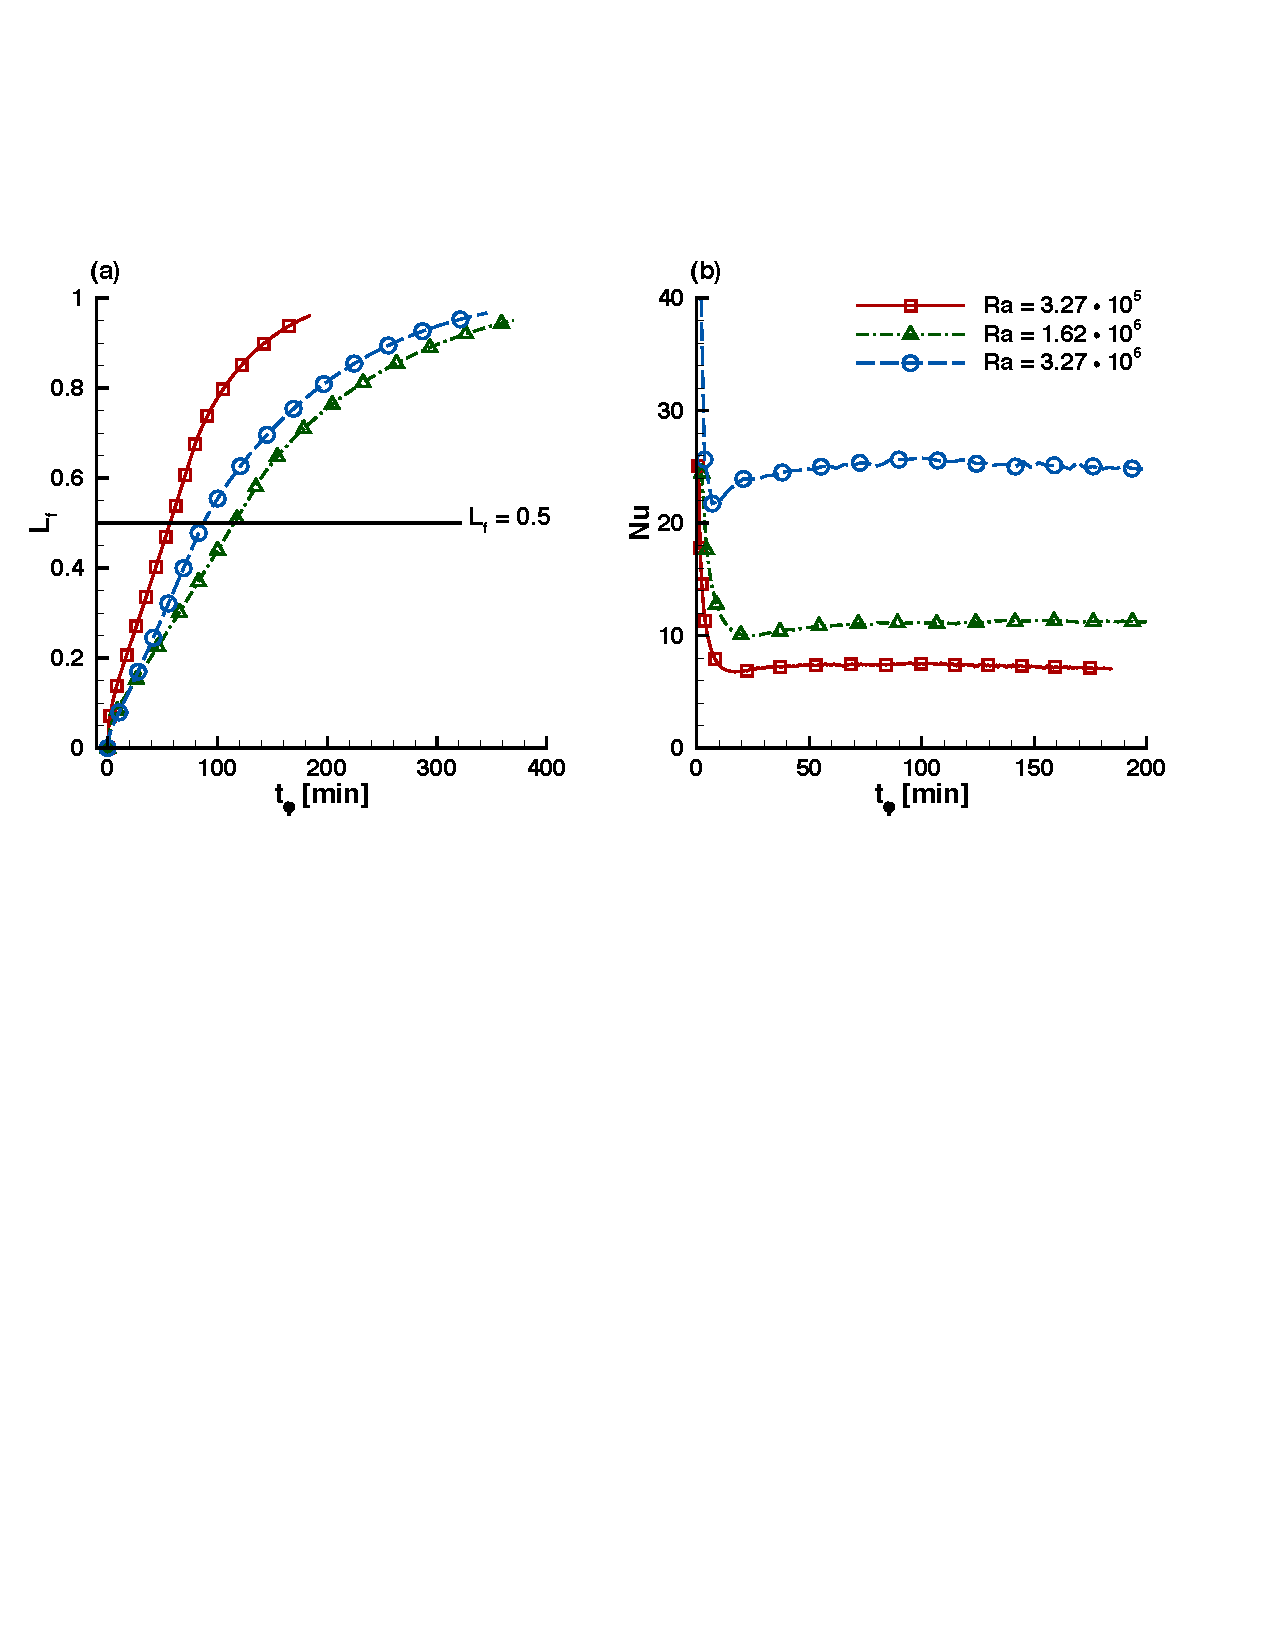
\includegraphics[width=.9\textwidth]{\figpath/Fig_cap_melting/fig08_2}
	\end{center}
	\caption{Complete melting of the PCM.  Influence of the value of the Rayleigh number ($\Ray$) on the time evolution of the liquid fraction (a) and the average Nusselt number defined at the hot (left) wall (b). The reference case ($\Ray=3.27\cdot 10^5$) is represented by red continuous lines. The value of the $\Ray$ was increased by a factor of $5$ and $10$, respectively while the Stefan number $\Ste$ is kept constant.}\label{fig:Ra-Nusselt-H}
\end{figure}

\begin{figure}
	\begin{center}
		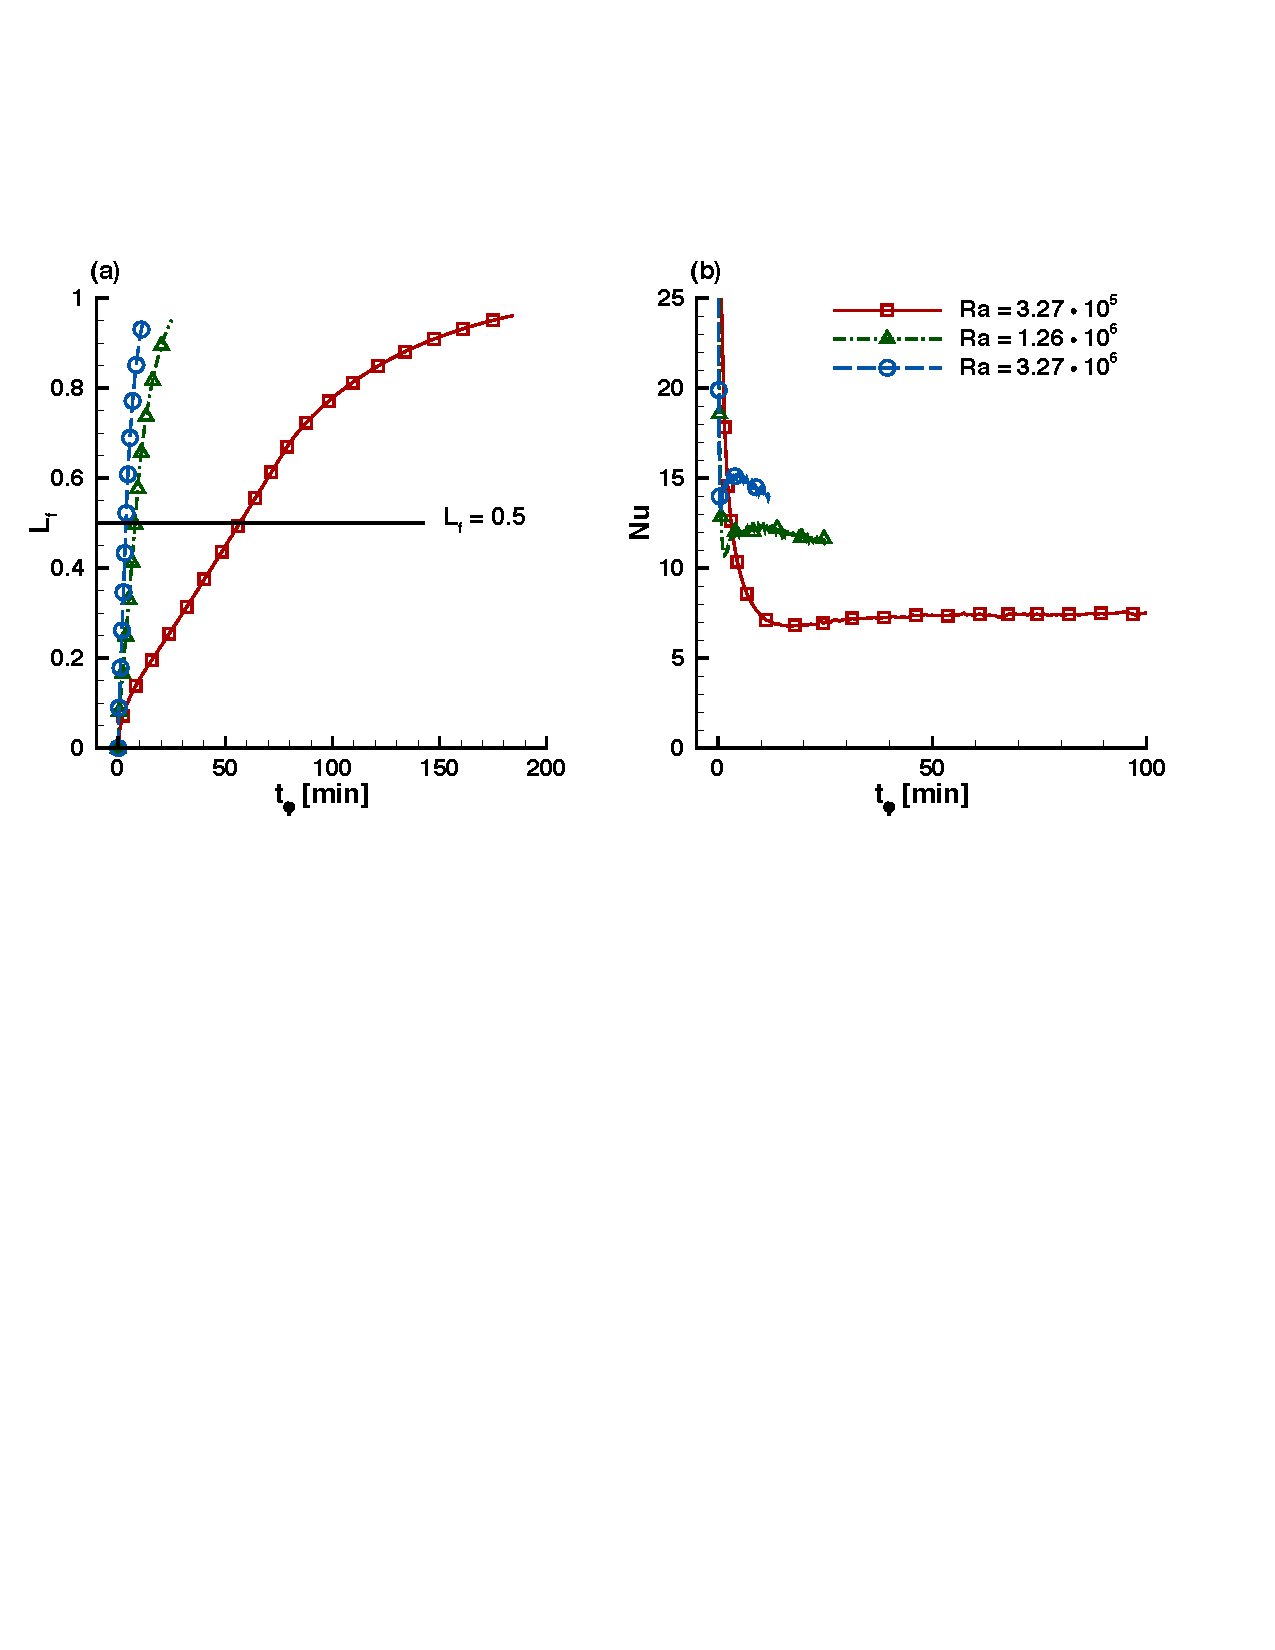
\includegraphics[width=.9\textwidth]{\figpath/Fig_cap_melting/fig09_2}
	\end{center}
	\caption{Complete melting of the PCM.  Influence of the value of the Rayleigh number ($\Ray$) on the time evolution of the liquid fraction (a) and the average Nusselt number defined at the hot (left) wall (b). The reference case ($\Ray=3.27\cdot 10^5$) is represented by red continuous lines. The value of the $\Ray$ and $\Ste$ were increased by a factor of $5$ and $10$, respectively.}\label{fig:Ra-Nusselt-deltaT}
\end{figure}

\newpage
\clearpage
\section{Basal Melting of n-octadecane PCM. Case BM} \label{sec-melting-basal}
\begin{figure}[!ht]
	\begin{center}
		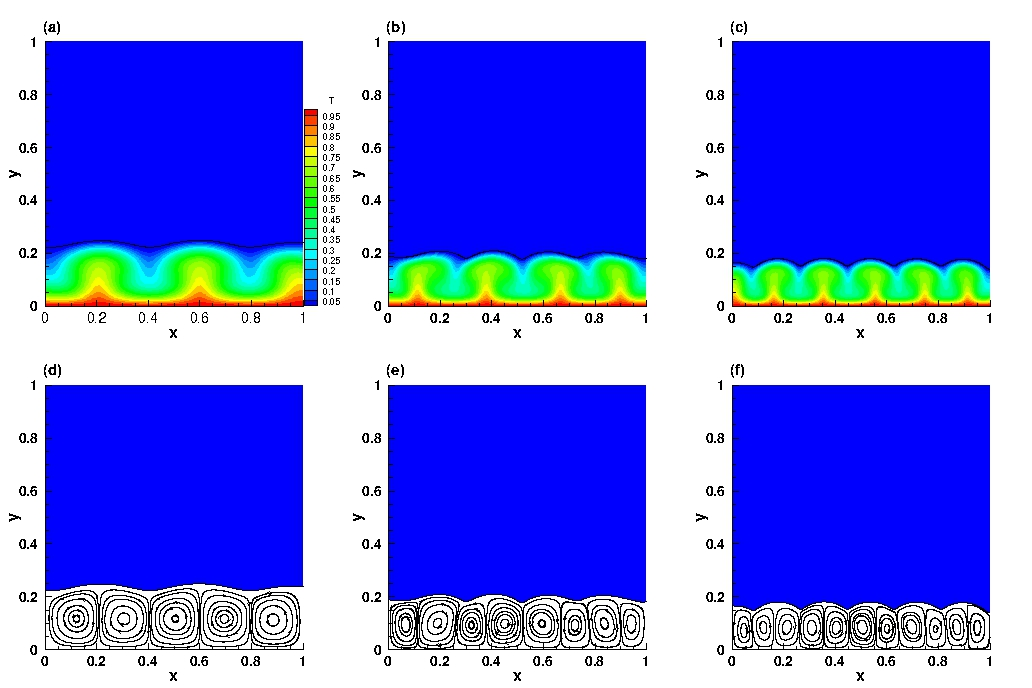
\includegraphics[width=\textwidth]{\figpath/Fig_cap_melting_basal/T_MELT_BASAL_heating_2}
	\end{center}
	\caption{Melting of PCM heated from below. (top) Temperature field and solid-liquid interface for different Rayleigh numbers (a) $\Ray = 3.27 \cdot 10^5$ and $t=30$, (b)  $\Ray = 1.635 \cdot 10^6$ and $t=15$, (c) $\Ray = 3.27 \cdot 10^6$ and $t=10$ (bottom) streamlines in the liquid phase.}
	\label{fig:melt-below}
\end{figure}

We now pay further attention to BM case.
We investigate the melting of pure n-octadecane PCM in a square enclosure subject to heating from the bottom side.
When compared to the lateral melting case, the dynamics of the melting is different for such configuration, in which natural convection develops in the form of B�nard cells. 
The physical parameters and the numerical configuration are reported in Fig. \ref{fig:melt-scheme}.
We perform two-dimensional numerical simulations, although 
 \cite{gau1983flow} and  \cite{gong1998flow} noticed the existence of three-dimensional convection cells during the very first step of the melting process.
These three-dimensional convection cells are however usually neglected for relatively moderate $\Ray$ numbers, particularly for $\Ray \leq 10^8$. 
In this case, three-dimensional cells survive over a very short duration compared to the whole melting process,
therefore the two-dimensional model is realistic.

\noindent A qualitative description of the dynamics of the natural convection flow and its impact on the melting front is first addressed in Sec. \ref{sec-RB-melt-process}.
Then, a scale analysis is conducted to describe the heat transfer that occurs during the melting in Sec. \ref{sec-RB-scal-analysis}.
Finally, a comparison between LM and BM cases is presented in Sec. \ref{sec-compare-LM-BM}.

\subsection{Temporal evolution of the melting process} \label{sec-RB-melt-process}
Figure \ref{fig:melt-below} displays the structure of the natural convection flow in the melting PCM through a sequence of panels for temperature isolines and streamlines in the liquid phase, for Rayleigh numbers ranging from $\Ray = 3.27 \cdot 10^5$ to $\Ray = 3.27 \cdot 10^6$, after the primary instability.
An array of lengthening plumes (panel a to c) and counter-rotating convective cells (panel d to f)  are located in the liquid phase,
in which the number of thermal plumes increases with the Rayleigh number.
For $\Ray = 3.27 \cdot 10^5$, one can observe three equidistant plumes and five convective cells in Figs. \ref{fig:melt-below}a and \ref{fig:melt-below}d, while four and six plumes are observed for $\Ray = 1.635 \cdot 10^6$ and $\Ray = 3.27 \cdot 10^6$ respectively (Figs. \ref{fig:melt-below}b and \ref{fig:melt-below}c).
These observations agree well with the numerical results of \cite{gong1998flow} and \cite{madruga2018dynamic} who studied the correlation between the number of thermal plumes and the size of the domain.
The shape of the interface is directly linked to the dynamics of these plumes.
The mushroom form of the plumes results from the two symmetric counter-rotating convective cells surrounding each of them.
We observe an anti-clockwise recirculation of the left convection cell and a clockwise recirculation of the right.
Thus, the melt is heated to the highest temperature at bottom and then floats up, reaches the phase change interface and splits into opposite directions.
The melt is cooled as it flows through the phase-change interface.
It results a non-planar front with a peak at the center of each couple of counter-rotating convective cells.

\noindent As the melting evolves, it is useful to introduce the effective Rayleigh and Nusselt numbers of the fluid layer, based on the height of the melted PCM, to describe the temporal evolution of the melting:
\begin{eqnarray}
	\Ray_{e} &=& \Ray \times {\bar \delta_H}^3, \\
	\Nuss_{e} &=& \Nuss \times \bar \delta_H ,
\end{eqnarray}
\noindent with ${\bar \delta_H}$ the non-dimensional averaged fluid height. Note that $\bar \delta_H $ could be assimilated to the liquid fraction.

Figure \ref{fig:T-evol-Ra-6.54e6} depicts in detail the temporal evolution of the melting for $\Ray = 6.54 \cdot 10^6$, during which the effective Rayleigh number increases and influences the dynamics of the flow. 
The temperature field, the location of the interface, and the streamlines are reported in panels (a) to (l).

\noindent Before the first instability arises, the melted layer evolves solely by conduction. 
There is no noticeable fluid flow and the melting front remains straight (panel a).
The temperature is distributed linearly in the vertical direction through the incipient liquid layer.
The convective onset occurs at $\Ray_e \approx 7 \times 10^3$ when the phase-change interface becomes non-planar (panel b), which is in good agreement with the observation of \cite{esfahani2018basal,favier2019rayleigh}.
It is worth noting that, in the framework of the classical Rayleigh-B�nard convection flow, the first instability appears at critical Rayleigh number $\Ray_c \approx 1707.76 $, in the limit of vanishing $\Ste$ number \citep{chandrasekhar2013hydrodynamic}.
This critical value is however higher for greater $\Ste$ numbers.
The appearance of convection is marked by a change in the shape of the interface from straight to nearly periodic curve.

\noindent  As the fluid expands upwards, the effective Rayleigh number increases and we could observe $10$ convective rolls being stretched vertically (panels c to e).
For $\Ray_e \leq 2 \cdot 10^5$, one can note that the number of rolls is time-independent.
Such behaviour could be compared to the steady convection regime after the onset of primary instability in the Rayleigh-B�nard system (see \cite{chandrasekhar2013hydrodynamic}).
This regime will be referred to linear regime in the present study.

\noindent After the rolls are elongated vertically, they start to oscillate laterally and then merge to create greater rolls, from $\Ray_e = 2.9 \times 10^5$ (panel g).
The interface loses periodicity and the structure of the rolls becomes disordered.
At this stage, neither the mushroom form of the plumes nor the periodic distribution of the convection cells are no longer observed. 
The essential consequence of this observation is that the melting front is modified.
The interface is actually shaped by the new flow pattern. 

\begin{figure}[!ht]
	\begin{center}
		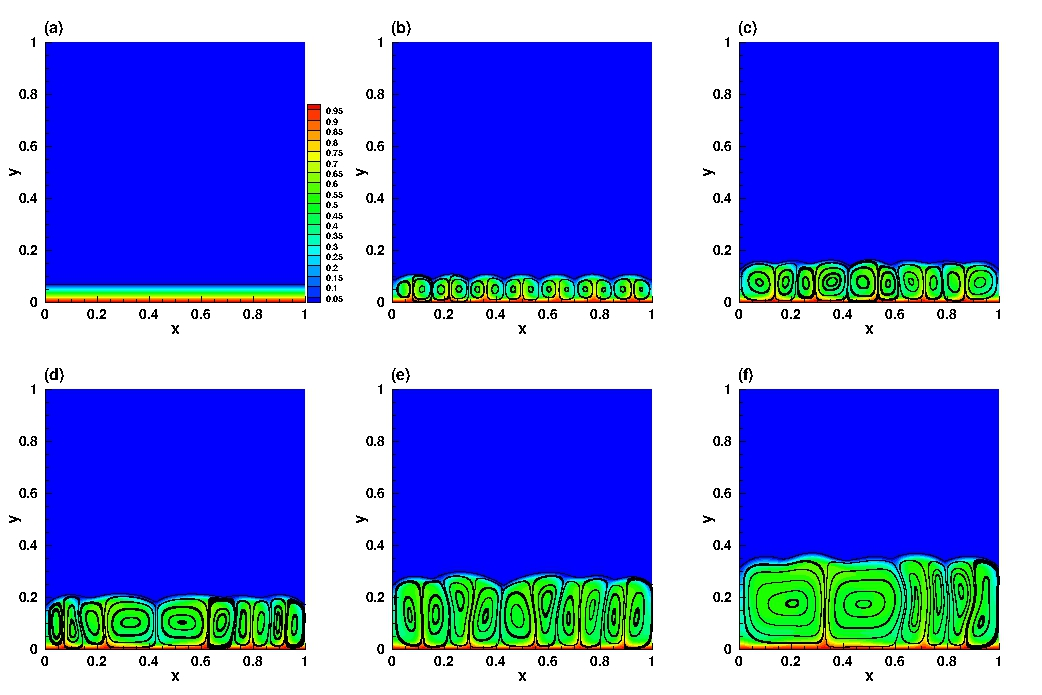
\includegraphics[width=\textwidth]{\figpath/Fig_cap_melting_basal/T_evol_654e6_1}
		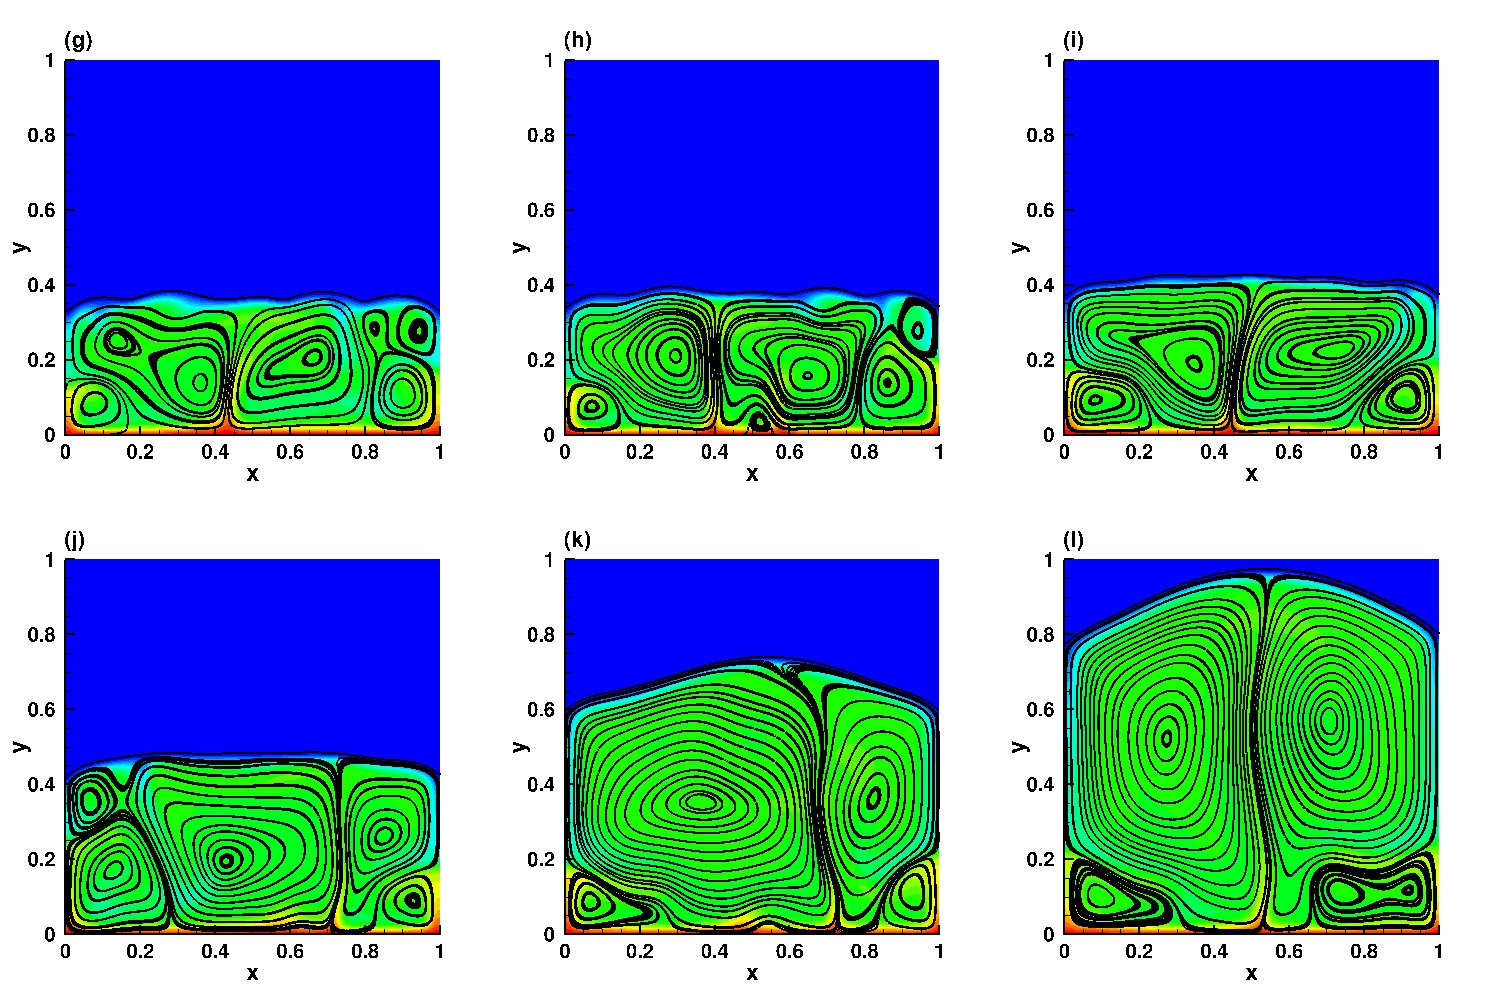
\includegraphics[width=\textwidth]{\figpath/Fig_cap_melting_basal/T_evol_654e6_3}
	\end{center}
	\caption{Melting of PCM heated from below: temperature field, solid-liquid interface and streamlines for several effective Rayleigh numbers. $\Ray = 6.54 \cdot 10^6$}
	\label{fig:T-evol-Ra-6.54e6}
\end{figure}


\subsection{Scale analysis} \label{sec-RB-scal-analysis}
Let us now proceed on a scale analysis for a comprehensive description of the heat transfer processes during the melting.
The dynamics of the BM case is usually classified into five regimes reported in the literature: a conductive regime, a linear regime, an oscillating regime, a turbulent regime, and finally an ultimate regime, defined following a power law of the $\mathcal{N}\!u - \Ray$ \citep{esfahani2018basal,madruga2018dynamic}.
The simulations performed in this chapter cover the first three regimes.
During the conductive regime, the heat transfer is fully dominated by the conduction. 
The time evolution of the liquid fraction and the Nusselt number could be approximated by the same scaling obtained in Eq. \eqref{eq-Nu-Lf-Corr-Lat}.
Notwithstanding, after the onset of the convection, the quasi-steady evolution of the heat transfer observed in the frame of LM case (see Fig. \ref{fig:Nusselt}), is no longer observed in BM case due to non-linear instabilities.

When the convective heat transfer is fully developed in the melted PCM, two distinct heat transfer processes could be identified:
a bulk heat transfer for low effective Rayleigh number regime, mainly for $\Ray_{e} \leq 10^5$,
followed by a boundary layer heat transfer regime, which is predominant when the flow becomes oscillatory or turbulent.
We develop in this section a scale analysis for the linear regime, during which bulk heat transfer occurs, to approximate the amount of heat transfer.
Beyond this regime, due to the important non-linearities of the dynamics, we rely on theories developed in the frame of turbulent Rayleigh-B�nard convection flow  \citep{malkus1954heat,grossmann2000scaling}. 
\begin{figure}
\centering
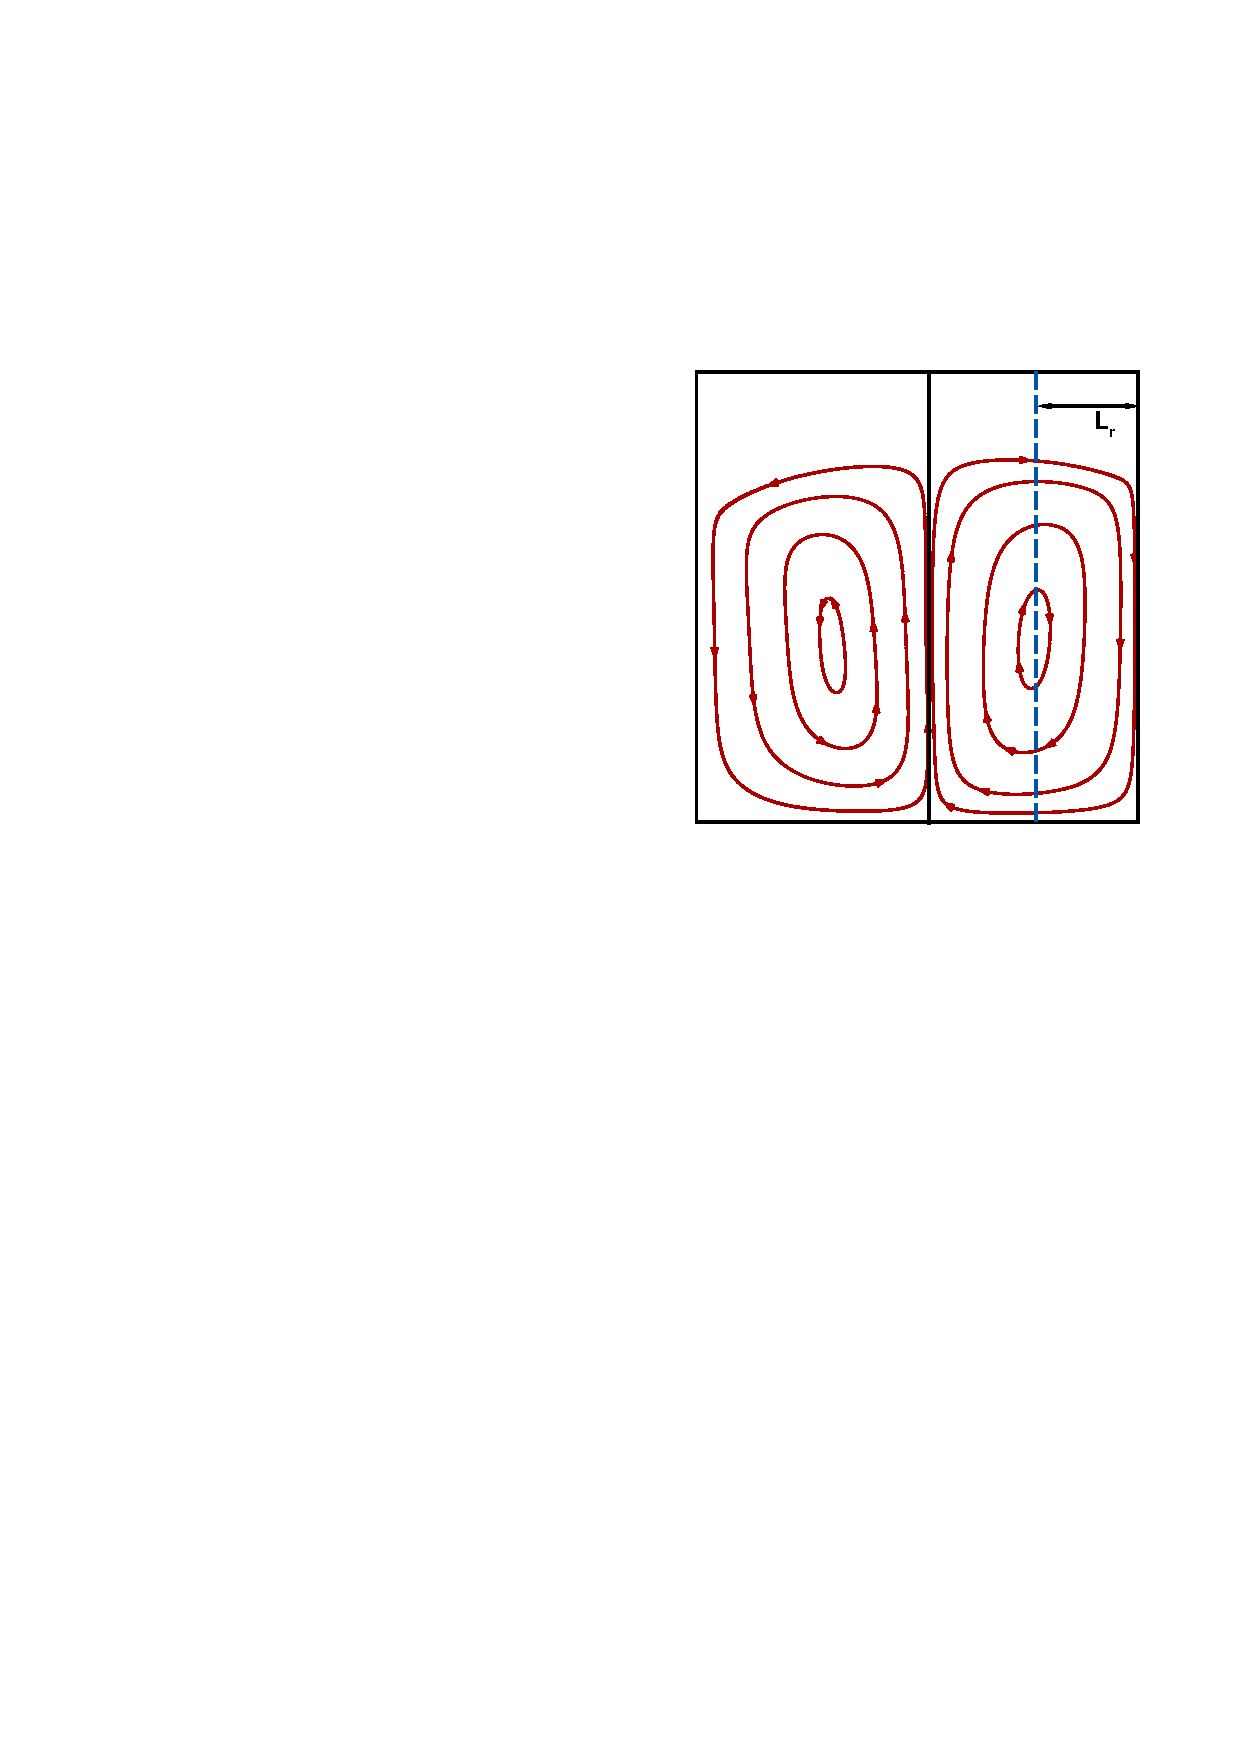
\includegraphics[width=0.5\textwidth]{\figpath/Fig_cap_melting_basal/MELT_basal_rolls}
\caption{Natural convection flow emerging from melting heated from below.}
\label{fig:roll-basal-heating}
\end{figure}

During the linear regime, the convective cells are elongated vertically and the number of rolls is time-independent.
In our scale analysis we will focus on a single roll convection pattern to assess the amount of heat transfer through it.
A schematic overview of the phenomenon is drawn in Fig. \ref{fig:roll-basal-heating}. 
Let us define $L_r$, the (dimensionless) half-thickness of a cell. 
An appropriate scaling during this regime is hence
\begin{equation}
	x \sim L_{r}, \quad y \sim \bar \delta_H,
\end{equation}

\noindent with $L_{r} < \bar \delta_H$.
We consider the dimensionless Navier-Stokes-Boussinesq system of Eqs. \eqref{eq-qmvt} - \eqref{eq-energ} applied to a single cell ($C=K=1$, and $S(\theta) = A(\theta) = 0$), which could be rewritten as follows (with scaling Eq. \eqref{eq-def-scal-1}, i.e. $\Rey = 1$):

\begin{eqnarray} \label{eq-mass-basal}
	\frac{\partial u}{\partial x} + \frac{\partial v}{\partial y} &=& 0, \\  \label{eq-mom-basal-x}
	\frac{\partial u}{\partial t} + u \frac{\partial u}{\partial x} + v \frac{\partial u}{\partial y} &=& - \frac{\partial p}{\partial x} +  \left( \frac{\partial^2 u}{\partial x^2} + \frac{\partial^2 u}{\partial y^2} \right), \\ \label{eq-mom-basal-y}
	\frac{\partial v}{\partial t} + u \frac{\partial v}{\partial x} + v \frac{\partial v}{\partial y} &=& - \frac{\partial p}{\partial y} +   \left( \frac{\partial^2 v}{\partial x^2} + \frac{\partial^2 v}{\partial y^2} \right) + \frac{\Ray}{\Prd} \theta, \\ \label{eq-bound-energy}
	\frac{\partial \theta}{\partial t} + u \frac{\partial \theta}{\partial x} + v \frac{\partial \theta}{\partial y} &=& \frac{1}{\Prd} \left( \frac{\partial^2 \theta}{\partial x^2} + \frac{\partial^2 \theta}{\partial y^2} \right). 	
\end{eqnarray}

\noindent The pressure $p$ is first eliminated by deriving Eq. \eqref{eq-mom-basal-x} with respect to $y$ and deriving Eq. \eqref{eq-mom-basal-y} with respect to $x$. One may refer to the book \cite{bejan2013convection} for more details, in the frame of the Rayleigh-B�nard convection flow.
Substracting one from the other, we get

\begin{eqnarray} \label{eq-mom-rassembly}
	\frac{\partial}{\partial y} \left( \frac{\partial u}{\partial t} + u \frac{\partial u}{\partial x} + v \frac{\partial u}{\partial y} \right) - \frac{\partial}{\partial x} \left(  \frac{\partial v}{\partial t} + u \frac{\partial v}{\partial x} + v \frac{\partial v}{\partial y} \right)  \\ \nonumber
	=  \left[ \frac{\partial}{\partial y} \left( \frac{\partial^2 u}{\partial x^2} + \frac{\partial^2 u}{\partial y^2} \right)   - \frac{\partial}{\partial x} \left( \frac{\partial^2 v}{\partial x^2} + \frac{\partial^2 v}{\partial y^2} \right) \right] - \frac{\Ray}{\Prd} \frac{\partial \theta}{\partial x}.
\end{eqnarray}

\noindent Since we have $L_{r} \ll \bar \delta_H$ (consequently $\partial^2 v/\partial y^2 \ll \partial^2 v/\partial x^2 $),
three terms are dominant in Eq. \eqref{eq-mom-rassembly}:
\begin{equation}
	\sim \underbrace{\frac{\partial ^2 v}{\partial x \partial t}}_{inertia}; \quad \sim \underbrace{ \frac{\partial^3v}{\partial x^3}}_{friction}; \quad \sim \underbrace{\frac{\Ray}{\Prd} \frac{\partial \theta}{\partial x}}_{buoyancy}.
\end{equation}

\noindent In terms of characteristic scales, this reduced momentum balance reads
\begin{equation} \label{eq-basal-heat-mom}
	\sim \underbrace{\frac{v}{L_{r} t}}_{inertia}; \quad \sim \underbrace{\frac{v}{L_{r}^3}}_{friction}; \quad \sim \underbrace{\frac{\Ray}{\Prd} \frac{\delta \theta}{L_{r}}}_{buoyancy},
\end{equation}

%\noindent with $\delta \theta \sim 1$. The linear regime occurs after a pure conductive regime where the boundary layer thickness increases as
%\begin{equation}
%	\delta_{\theta} \sim \left( \frac{t}{\Prd} \right)^{1/2}.
%\end{equation}
%
%\noindent Since the heat transfer is dominated solely by bulk heat transfer we have
%\begin{equation} \label{eq-Lf-deltT}
% 	L_{r} \sim \delta_{\theta}.
% \end{equation}
% 
\noindent Equation \eqref{eq-basal-heat-mom} could be hence simplified by normalising Eq. \eqref{eq-basal-heat-mom} with respect to the friction scale, leading to
\begin{equation}
	\underbrace{\frac{1}{\Prd}}_{inertia} \quad \underbrace{1}_{friction}  \quad \underbrace{\frac{\Ray L_{r}^2}{v \Prd}}_{buoyancy}.
\end{equation}

\noindent For high-Prandtl fluid, the momentum balance is between buoyancy and friction (see e.g. \cite{bejan2013convection,le1999note}) and we obtain
\begin{equation}\label{eq-scaleV}
	v \sim \frac{\Ray L_{r}^2}{\Prd}.
\end{equation}

\noindent Next, we turn attention back to the energy Eq. \eqref{eq-bound-energy}. During the pure conductive regime, the velocity is very small and negligible. The characteristic scale is therefore:

\begin{equation}
	\frac{\delta \theta}{t} \sim \frac{\delta \theta}{\Prd L_r^2}
\end{equation}

\noindent leading to

\begin{equation}
	L_r \sim \left( \frac{t}{\Prd} \right)^{1/2}.
\end{equation}

\noindent At this earlier stage, the thermal layer thickness is of the same order as $L_r$, $\delta_{\theta} \sim L_r$. When the melting evolves (i.e. time increases), the inertia decreases in importance. 
When the convection arises, we can identify three distinct effects
\begin{equation}
	\underbrace{\frac{1}{t}}_{Inertia} \quad \underbrace{\frac{v}{\bar \delta_H}}_{Convection} \quad \underbrace{\frac{1}{L_r^2 \Prd}}_{Conduction}.
\end{equation}

\noindent There comes an effective time $t_{e}$ where the energy equation expresses a balance between the convection and the conduction heat transfer (see \cite{bejan2013convection}):

\begin{equation} \label{eq-scale-v-deltaH}
	 \frac{v}{\bar \delta_H} \sim \frac{1}{\delta_{\theta}^2 \Prd}.
\end{equation}

\noindent Equations \eqref{eq-scale-v-deltaH} and \eqref{eq-scaleV} lead to

\begin{equation}
	\frac{\delta_H}{\delta_{\theta}^2 \Prd} \sim \frac{\Ray \delta_{\theta}^2}{\Prd},
\end{equation}

\noindent  since $\delta_{\theta}^2 \sim t/\Prd$, we have

\begin{equation}
	t_{e} \sim \left( \frac{\bar \delta_H}{\Ray_e} \right)^{1/2} \times \Prd.
\end{equation}

\noindent At this effective time $t_e$, during which the inertia becomes negligible, and the convection effects increases, the thermal layer thickness is
\begin{equation}
	\delta_{\theta} \sim \left(\frac{t_{e}}{\Prd} \right)^{1/2} \sim \left(\frac{\bar \delta_H}{ \Ray_{e}}\right)^{1/4} \sim \left( \bar \delta_H \right)^{-1/2} \Ray^{-1/4}.
\end{equation}

\noindent Accordingly, before the flow oscillates, the scaling for $\Nuss$ could be written as

\begin{equation} \label{eq-Nu-scal-basal}
	\Nuss \sim  \bar \delta_H ^{1/2} \times \Ray^{1/4}.
\end{equation}

\noindent Equation \eqref{eq-Nu-scal-basal} highlights that the heat transfer through a single convection cell depends on the height of the melted PCM layer during the linear regime.
Correlations pertaining to basal melting case in the literature do not distinguish between this contribution of the bulk and the boundary layer heat transfers after the onset of convection and relies directly on empirical correlations for turbulent Rayleigh-B�nard flows.
It should be noted that Eqs. \eqref{eq-Nu-scal-basal} rely on only one cell in the system. 

\noindent The exponents of the power laws obtained by our numerical simulations for four Rayleigh numbers are given in Tab. \ref{tab-power-expo} during the linear and the oscillating regime.
An exponent of $0.28$ is observed for the linear regime and decreases with increasing Rayleigh number, which overestimates slightly the predicted scaling exponent of $1/4$.
This is mostly due to the number of convection cells in the melted PCM and the effect of the non-planar solid-liquid interface, not taken into account in our analysis.
However, our numerical results match better with the Grossmann-Lohse theory \citep{grossmann2000scaling}, which predicts a scaling exponent of $2/7$, within the framework of natural convection flow.
Furthermore, during the oscillating regime the exponent increases with the Rayleigh number and tends to the empirical exponent of $1/3$.

\noindent Figure \ref{fig:NU-LF-evol}a plots the temporal evolution of the heat flux, represented by the Nusselt number, and the strength of buoyancy, represented by the Rayleigh number, when the melting evolves.
The onset of the convection arises around $\Ray_e = 2 \times 10^3$, when a sudden jump in the evolution of $\Nuss_e$ is observed.
\cite{vasil2011dynamic} have investigated a weakly non-linear stability analysis and have highlighted a superexponentional amplitude growth when the Rayleigh number becomes close to the traditional critical value in the limit of vanishing Stefan number.
This superexponential growth is moreover followed by a rapid pattern readjustment.
The trend of $\Nuss_e$ at the onset of convection is in total accordance with the prediction of \cite{vasil2011dynamic}.
The results of \citep{esfahani2018basal,madruga2018dynamic,favier2019rayleigh} exhibit the same trend despite the different boundary conditions (periodic lateral boundary conditions, adiabatic boundary conditions at the top of the cavity, and low value of $\Prd$ for \cite{esfahani2018basal} and \cite{favier2019rayleigh}).
The rapid growth of $\Nuss_e$ is followed by a power law with averaged exponent $\Nuss \sim \Ray^{0.28}$ for  $10^3 \leq \Ray \leq  10^5$.
Finally, the transition from steady pattern of the convective rolls, to oscillating pattern, followed by cell merging, as it is clearly shown in Fig. \ref{fig:T-evol-Ra-6.54e6}(d-f), 
is also illustrated by a decrease of $\Nuss$ at $\Ray \sim 10^5$, followed by high oscillation in the temporal evolution of the heat transfer.
The power-law relation $\Nuss-\Ray$ is bounded in this stage by the average exponent of $1/3$.

\begin{table}[!ht]
   \begin{center}
      \begin{tabular}{*{3}{cl}}
         $\Ray$ & Linear regime & oscillating regime \\
         \bottomrule
         $3.27 \cdot 10^5$ & $0.286299$ & - \\
         $1.635 \cdot 10^6$ & $0.274789$ & 0.269158 \\
         $3.27 \cdot 10^6$ & $0.279616$ & 0.283658 \\
         $6.54 \cdot 10^6$ & $0.274043$ & 0.294528 \\
      \end{tabular}
   \end{center}
   \caption{Exponent of the power laws of the linear and the oscillating regimes.}
   \label{tab-power-expo}
\end{table}

As far as the temporal evolution of the liquid fraction $L_f$ is concerned, one can introduce the following scaling, from \cite{favier2019rayleigh}, obtained by a balance between the total rate of change of the enthalpy in the system and the heat fluxes entering and leaving the domain:
\begin{equation}\label{eq:scal-Lf-RB}
	L_f(t) = \left[ \sqrt{2 t}^{(2-3 \beta)}+ c \Ray^\beta t \right]^{1/(2-3 \beta)},
\end{equation}
with $\beta$ the exponent in the $\Nuss-\Ray$ power law, $c = \frac{(2-3 \beta) \gamma}{2 + \Ste}$ and $\gamma$ a constant fitted from numerical data.

\noindent The time evolution of the liquid fraction is illustrated in Fig. \ref{fig:NU-LF-evol}b.
As expected, the purely diffusive stage displays the scaling $L_f \sim t^{1/2}$.
Replacing $\beta$ by the exponent value $2/7$ observed in our numerical simulations, we obtain $L_f \sim t^{7/8}$.
Our simulations exhibit a power-law evolution of $L_f \sim t^{0.82}$ when the convection is fully developed in the fluid, corresponding to $\Ray_e \geq \Ray_c$.

\begin{figure}
	\begin{center}
		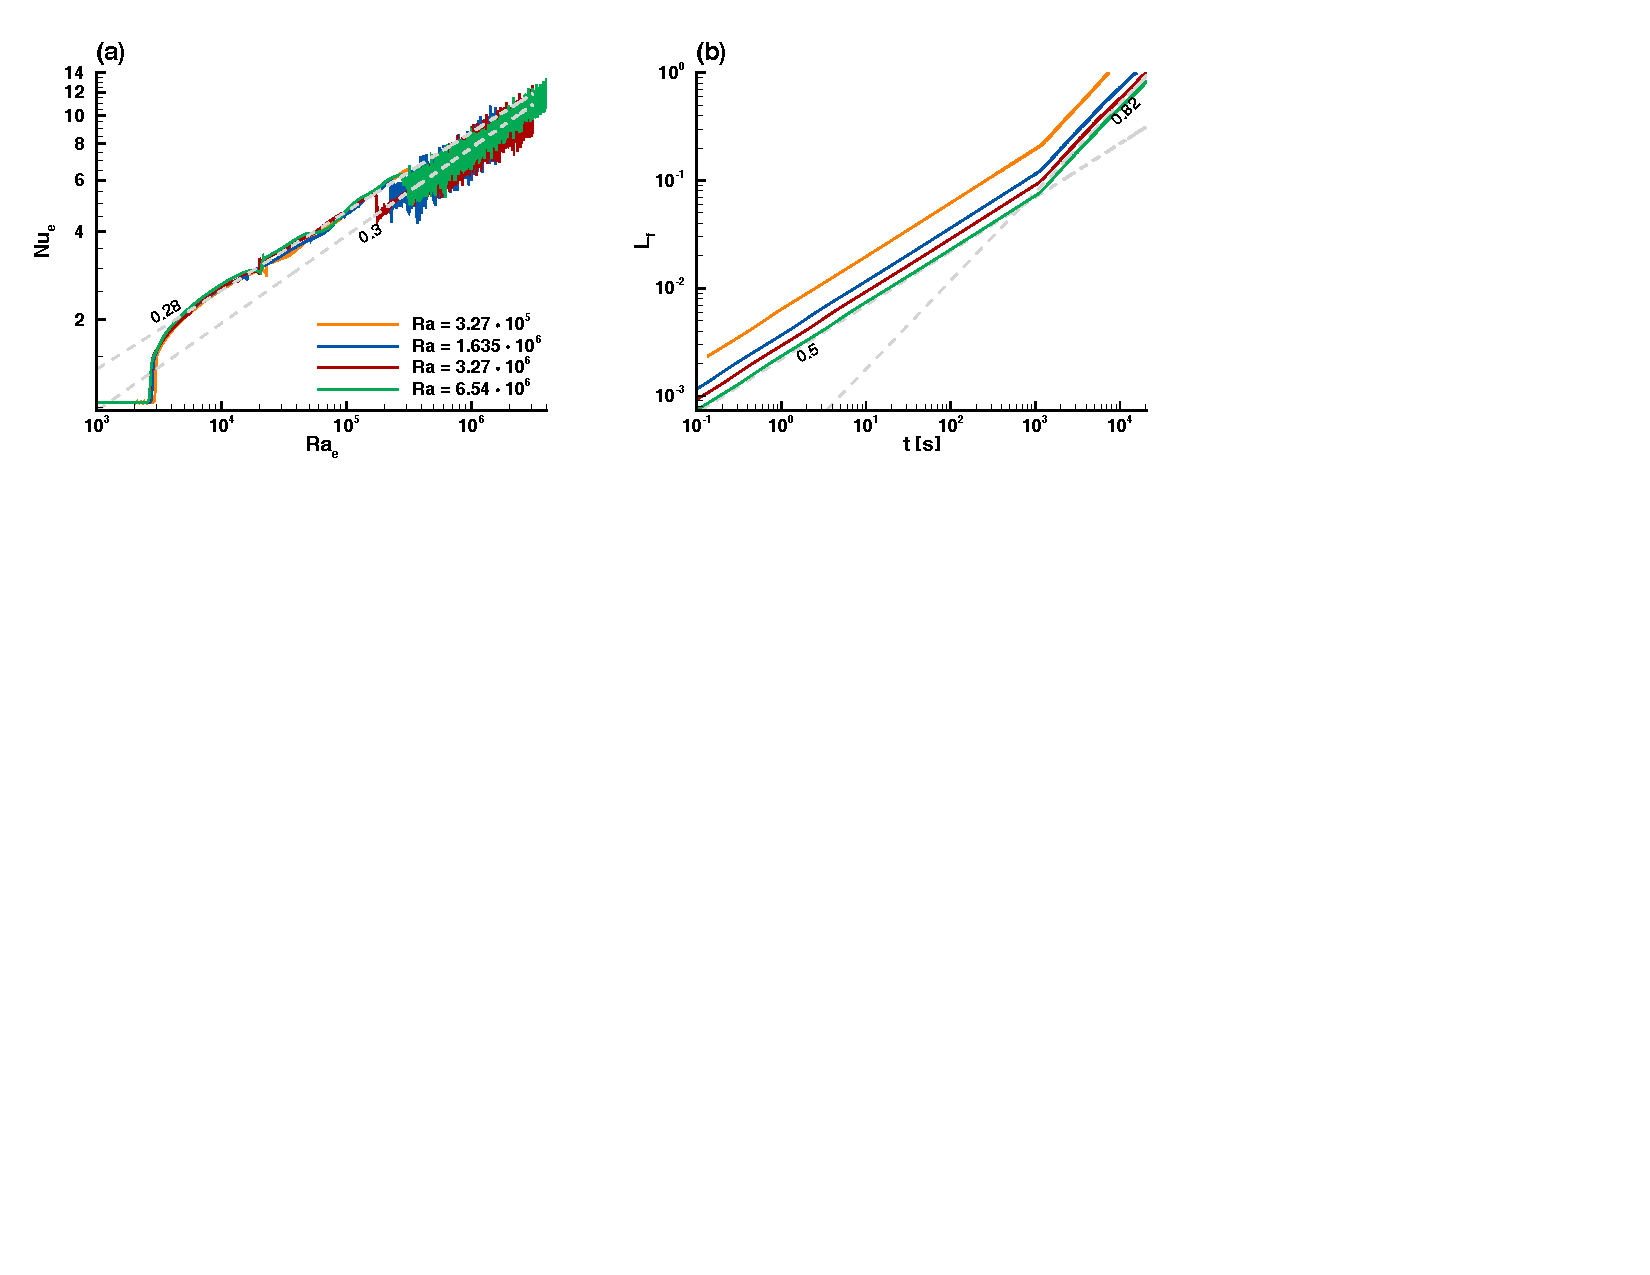
\includegraphics[width=\textwidth]{\figpath/Fig_cap_melting_basal/NU-LF-PHYS_2}
	\end{center}
	\caption{BM case for three Rayleigh numbers: $\Ray = 3.27 \cdot 10^5$, $1.62 \cdot 10^6$, and $3.27 \cdot 10^6$. Time evolution of the Nusselt number (a) and the melting rate (b).}
	\label{fig:NU-LF-evol}
\end{figure}


\section{Comparison between LM and BM cases} \label{sec-compare-LM-BM}
%We now compare the temporal evolution of some physical quantities for both LM and BM cases.
A comparison of the liquid fraction $L_f$, the Nusselt number $\Nuss$, and the accumulated heat input $Q_0$ is offered in Fig. \ref{fig:NU-LF-Q0-compare}. 
Blue lines denote the LM case and red lines the BM case.
Different values of the $\Ray$ number, ranging from $\Ray = 3.27 \cdot 10^5$ to $\Ray = 6.54 \cdot 10^6$ are investigated.

The temporal evolution of $L_f$ (left panels) displays a similar trend of both curves up to $L_f = 0.6$ for all cases. 
For instance, for $\Ray = 3.27 \cdot 10^5$ (panel a), LM and BM cases evolve at the same rate from $t=0$ to $t=100$, corresponding to $60 \%$ of melted PCM.
Then, for greater Rayleigh numbers, the gap keeps increasing, albeit slightly.
This result agrees with the scaling analysis that predicts the same trend of both systems as long as the number of convective cells is close to one.
Since the number of rolls is increasing with the Rayleigh number, an enhancement of the melting rate is thus consistent.
Furthermore, differences are noticeable for $L_f \geq 0.6$, when the interface of LM case reaches the right (cold) interface.
Increasing the Rayleigh number induces actually a faster advancement of the top of the LM front, which touches the cold wall earlier, slowing hence the evolution of the melting.
One can observe during this period a decrease of the slope of the blue curve with respect to the vertical axis.
Linear evolution of $L_f$ is however noticed throughout the basal melting time since the interface touch the top cold wall very late. 
%One can see a decrease of the slope of the red curve in when the PCM is almost liquid with $L_f = 0.95$.


Regarding the time evolution of the heat transfer (middle panels), red and blue curves matche perfectly well during the conductive regime (see for e.g. Fig. \ref{fig:NU-LF-Q0-compare} from $t=0$ to $t=18$ for $\Ray = 3.27 \cdot 10^5$). 
It is obviously expected since the contribution of the convective heat transfer is still negligible at this stage.
Differences occur from the emergence of the natural convection flow.
The evolution of $\Nuss$ is relatively smooth for LM case, while the BM case exhibits a sudden increase due to the hydrodynamical instabilities. 
Significant gap between both curves arises during the oscillating regime: $\Nuss$ displays a highly oscillating value for the BM case when the liquid layer expands upward, while the LM case reaches an asymptotic value.
It is worth noting that for higher and higher Rayleigh numbers, the Nusselt number increases accordingly.

The evolution of the accumulated heat input $Q_0$ is consistent with the foregoing remarks.
$Q_0$ is defined as follows:
\begin{equation}
    Q_0 = \int_0^{t_{\varphi}} N\!u \, d t_{\varphi},
    \label{eq-Q0}
\end{equation}
with $t_{\varphi}$ the physical time.
The decrease of the heat transfer monitored by the cell merging process in the BM case leads to a lower accumulated heat input.
It occurs when the heat transfer is no longer bulk transfer for the BM case.
It follows that a more important thermal energy is stored with respect to the LM case.

These observations are of particular importance for PCM design for a specific application.
If a fast melting is sought, BM case is advised. It could be the case for example during quick temperature peak in electronic components.
Conversely, when the PCM is expected to melt in longer period, LM case is appropriate.

\begin{figure}
	\begin{center}
		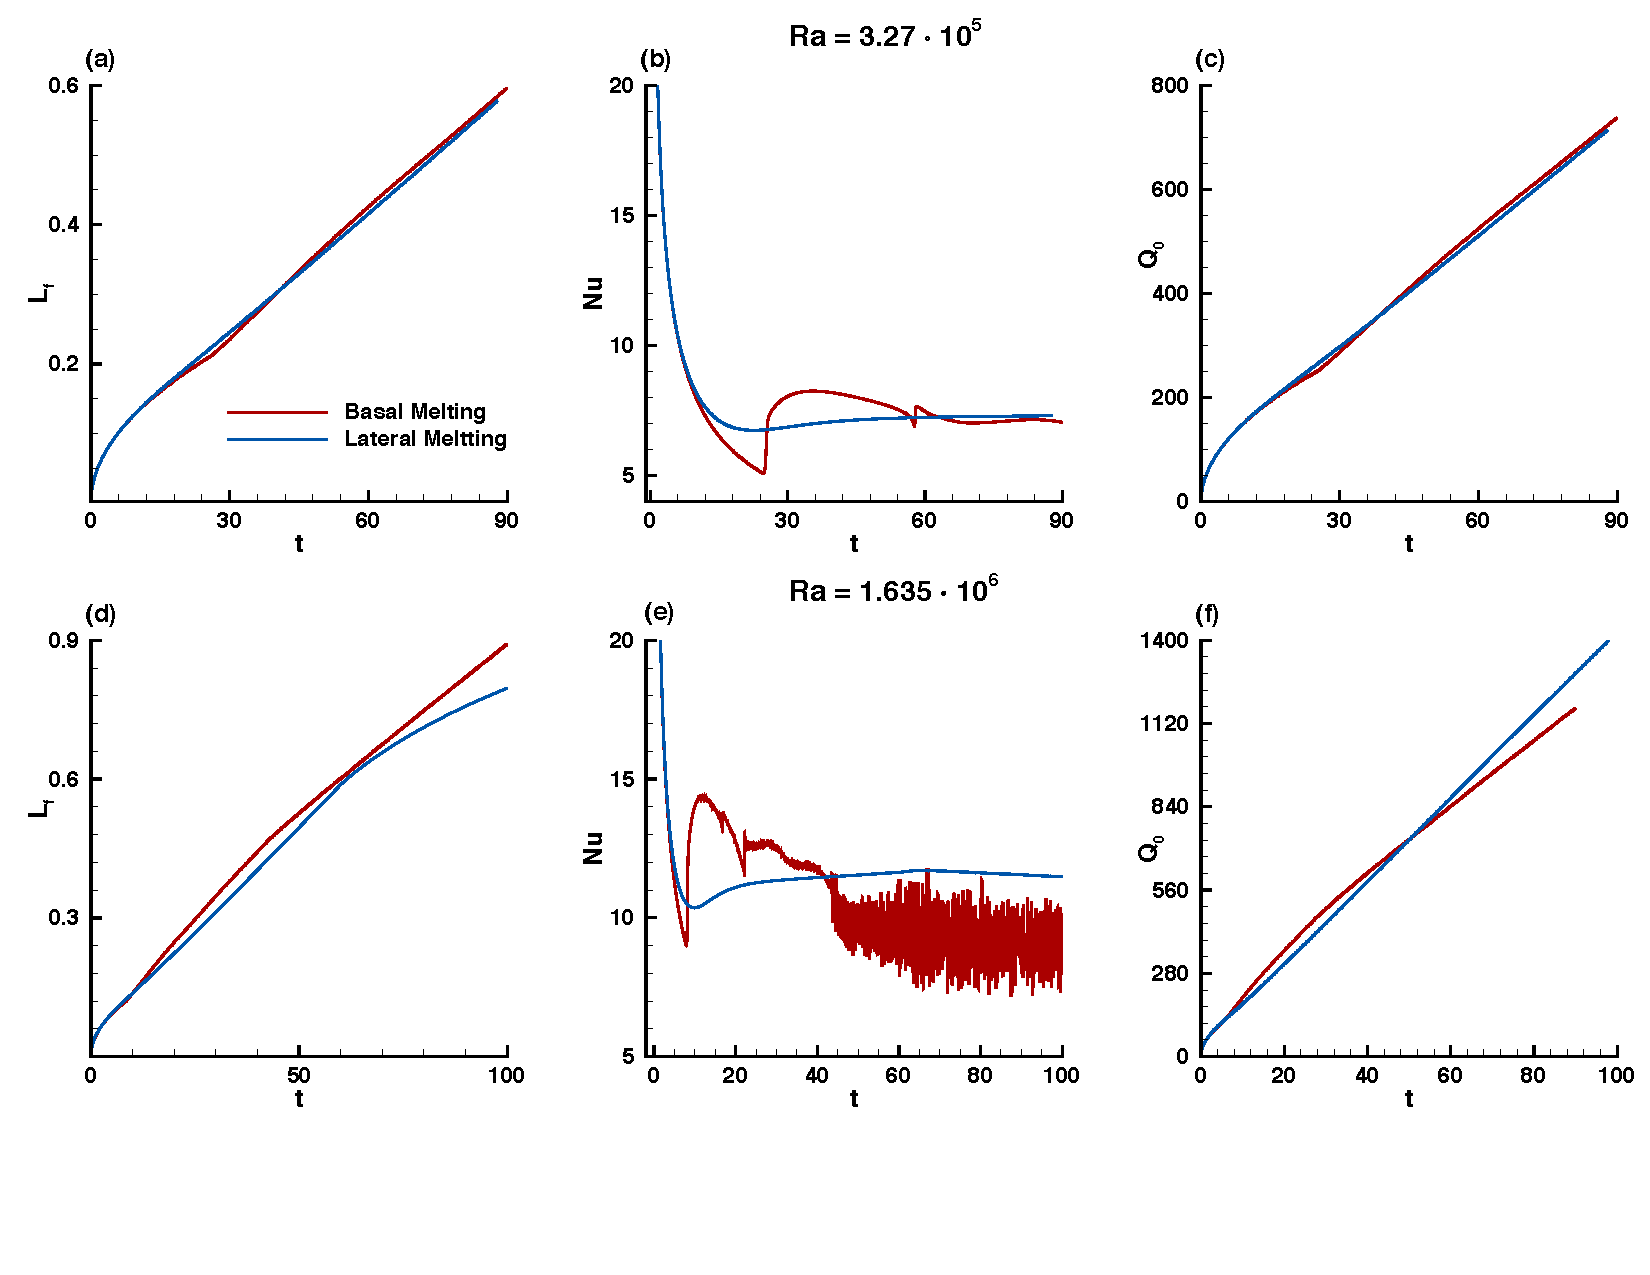
\includegraphics[width=\textwidth]{\figpath/Fig_cap_melting_basal/NU-LF-Q0_1}\\
		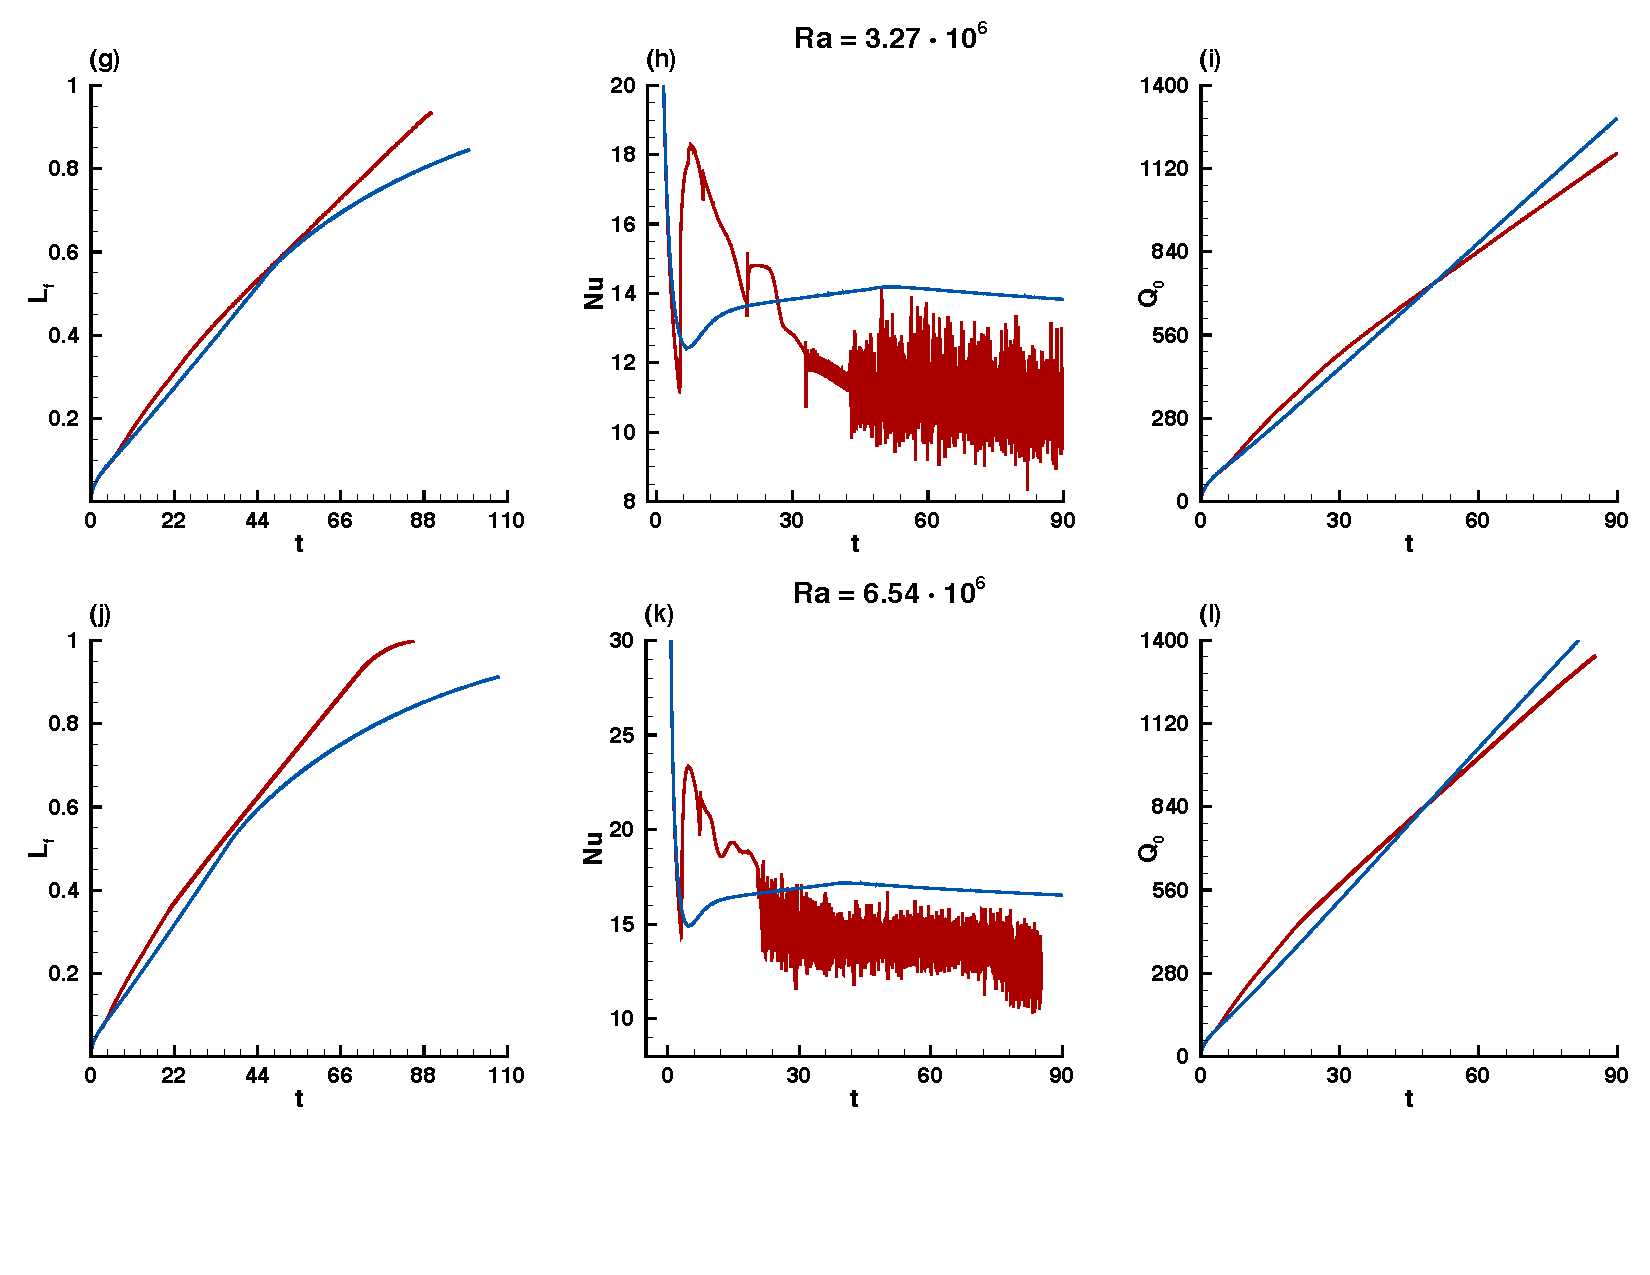
\includegraphics[width=\textwidth]{\figpath/Fig_cap_melting_basal/NU-LF-Q0_2}
	\end{center}
	\caption{Comparison between LM and BM cases. Rayleigh number ranging from $\Ray = 3.27 \cdot 10^5$ to $\Ray = 6.54 \cdot 10^6$. (left) Liquid fraction, (middle) Nusselt number, and (right) accumulated heat input.}
	\label{fig:NU-LF-Q0-compare}
\end{figure}

\section{Concluding remarks}
The high accuracy of our numerical method has permitted to simulate in this chapter lateral and basal melting case.
Numerical and theoretical comparisons of both cases were performed and have exhibited many differences, mainly on the dynamics of the flow and the heat transfer processes.
A main question related to convective melting processes in all their generality is however the prediction of the temporal evolution of the melting rate, which is correlated to the heat-flux dynamics determined by the flow in the system.
Since the dynamics of the flow is completely different for LM and BM systems, we have performed simulations for both cases and compared the evolution of some physical parameters.  

We have investigated first the LM case, by simulating the melting of n-octadecane inside a square enclosure heated from the vertical wall.
Three principal regimes were identified to describe the dynamics of the melting: conductive regime, mixed regime, and convective regime.
The influence of the Rayleigh and the Stefan parameters on the flow was also assessed and have indicated clearly that increasing $\Ray$, by increasing either $H$ or $\delta T$, enhances the heat transfer.
Since stronger convection flow occurs in the liquid region with increasing Rayleigh number, the shape of the phase-change front is altered consequently.
The top of the interface moves faster while the bottom part is rather slowed, resulting in a curved shape of the melting front.

Concerning the simulations of BM case, a large range of Rayleigh numbers, ranging from $\Ray = 3.27 \cdot 10^5$ to $\Ray = 6.54 \cdot 10^6$ were carried out for a comprehensive description of the dynamics of the melting.
Effective Rayleigh and Nusselt numbers, depending on the fluid height were introduced to describe the flow.
The melted fluid layer was shown to be thermally unstable and quickly develops convective motion of progressively higher intensity as the depth of the melted layer increases.
The onset of these instabilities were observable either on the dynamics of the melting flow or the temporal evolution of Nusselt number.
The novelty is the theoretical description of the convective heat transfer during the linear regime, i.e $\Ray_e \leq 10^5$, through a scale analysis by separating the contribution of the bulk and the boundary layer heat transfers.
For higher $\Ray_e$ numbers, we used the knowledge acquired on turbulent natural convection system, to understand convective melting.

We have finally compared the time evolution of the liquid fraction $L_f$, the heat transfer rate represented by the $\mathcal{N}\!u$ number, and the accumulated heat input $Q_0$, and have shown that PCM melts faster when heated from below compared to the lateral melting, since the last case reaches the cold wall earlier, slowing accordingly the melting rate.
However, the lateral oscillation of the convective cells in BM case, yielding to cell merging processes, reduces the heat transfer rate.
In the following chapter, we investigate the full melting-solidification cycle in the next chapter for a better understanding of the complete PCM cycle.



